\documentclass[12pt]{article}
\usepackage{amsmath}
\usepackage{graphicx}
\usepackage{enumerate}
\usepackage{natbib}
\usepackage[T1]{fontenc}
\usepackage[latin9]{inputenc}
\usepackage{color}
\usepackage{float}
\usepackage{hyperref}
\usepackage{multirow}
%\usepackage{babel}

\newcommand{\blind}{0}

\addtolength{\oddsidemargin}{-.75in}%
\addtolength{\evensidemargin}{-.75in}%
\addtolength{\textwidth}{1.5in}%
\addtolength{\textheight}{1.3in}%
\addtolength{\topmargin}{-.8in}%

\makeatletter

%%%%%%%%%%%%%%%%%%%%%%%%%%%%%% LyX specific LaTeX commands.
%% Because html converters don't know tabularnewline
\providecommand{\tabularnewline}{\\}

\newcommand{\red}[1]{{\color{red} #1}}

\makeatother

\begin{document}

\def\spacingset#1{\renewcommand{\baselinestretch}%
{#1}\small\normalsize} \spacingset{1}

%%%%%%%%%%%%%%%%%%%%%%%%%%%%%%%%%%%%%%%%%%%%%%%%%%%%%%%%%%%%%%%%%%%%%%%%%%%%%%

\if0\blind
{
  \title{\bf  Enabling Interactivity on Displays of Multivariate Time Series and Longitudinal Data}
  \author{Xiaoyue Cheng,
    Dianne Cook, Heike Hofmann \\
    Department of Statistics, Iowa State University
    }
\date{}
  \maketitle
} \fi

\if1\blind
{
  \bigskip
  \bigskip
  \bigskip
  \begin{center}
    {\LARGE\bf Enabling Interactivity on Displays of Multivariate Time Series and Longitudinal Data}
\end{center}
  \medskip
} \fi

\bigskip
\begin{abstract}
Temporal data is information measured in the context of time. This contextual structure provides components that need to be explored to understand the data and that can form the basis of interactions applied to the plots. In multivariate time series we expect to see temporal dependence, long term and seasonal trends and cross-correlations. In longitudinal data we also expect within and between subject dependence. Time series and longitudinal data, although analyzed differently, are often plotted using similar displays.  We provide a taxonomy of interactions on plots that can enable exploring temporal components of these data types, and describe how to build these interactions using data transformations. Because temporal data is often accompanied other types of data we also describe how to link the temporal plots with other displays of data. The ideas are conceptualized into a data pipeline for temporal data, and implemented into the R package \texttt{\textbf{cranvas}}. This package provides many different types of interactive graphics that can be used together to explore data or diagnose a model fit.

%Exploring temporal data can be facilitated by interactive graphics that allow structural components of the data to be sliced, diced and rearranged. This paper explains how to build upon static displays, to create interactive graphics. This involves developing a taxonomy of desirable tasks, restructuring data, and conceptualization of a data pipeline to realize the interactions.

%We describe structuring data objects to support different types of temporal displays. A taxonomy of interactions is given that can be useful for examining different components of multivariate time series and longitudinal data: seasonality, temporal dependence, cross-correlation, within and between subject variation. The conceptual data pipeline framework for realizing the interactions using primarily data transformations is explained. The ideas are implemented in the R package \texttt{\textbf{cranvas}}, which is a system for exploring data using multiple linked windows. The way the temporal displays are linked to displays of other variables as part of a general interactive graphics system is explained.
\end{abstract}

\noindent%
{\it Keywords:}  Interactive graphics; Multivariate time series;
Longitudinal data;  Multiple linked windows; Data visualization; Statistical graphics.

\spacingset{1.45}

\section{Introduction}

Constructing interactive graphics for temporal data can be enabled by building upon static displays. Aspects of the graphical elements in the displays can be made accessible to modification by user actions, for the purpose of facilitating different exploration of the temporal components in the data. To explain how to do this we first need to understand how time might be structured, and the common types of temporal data displays.

%Interactions would change the static pictures by some order such that the user can find the best graphical summary. Hence before introducing the interactive graphics, we give an overview of the static graphics for temporal and longitudinal data in this section.


\subsection{Characterizing time}

In data, time is coded in many different ways: as a date/time format ("Wed Oct 15 09:51:53 2014"), as discrete or continuous values, sporadic events or intervals. Recoding a time variable into other units like week in the year or days in the month, although convenient for some tasks, brings imprecision, as do events like leap years, and seconds. There may not be a well-defined absolute time line, and periodicity can be hard to quantify. Variables measured over time may be measured on different scales, e.g. atmospheric particulate matter and mortality might be drawn from different sources to study the effect of pollution on human health and measured at different resolutions.

%The custom time formats brings some further problems, for example, the number of weeks per year is not an integer, the number of days per month varies over the year, and the leap year recurs every four years. In some cases, the data can only be collected during the weekdays.  Therefore, the time plot may not be accurate in an absolute time line, and the length of the periodicity could be hard to verify. Besides, the dependent variables could appear with different time formats, which makes the visualization more difficult but interesting.

The most common description of time is as a continuous or discrete ordered numerical variable. All data is technically discrete, but if measurements are recorded often enough, and long enough they are effectively continuous. For example, currency exchange rates change on a microsecond basis, blood pressure measurements made with a wearable device records at every minute. For these examples time could essentially be considered continuous. However, it may be not helpful to evaluate trends on this microscale, and aggregating at an hourly, daily or monthly value may be sufficient. For simplicity, the methods developed in this paper assume the time variable is measured on a discrete scale.
%The main division of the data types is that whether the time is discrete or continuous. For example, the time to record the salary of an employee is discrete, but the time for the temperature in a location is continuous. However, people can not measure a variable continuously over time, so the data collected is still discrete. To simplify the problem, we only consider the discrete case. Another further division of the discrete time series data is that whether a time datum is recorded as an event or an interval. For example, in a customer visiting problem, the time length that each customer stays  (interval) is as important as the time that the customer enters  (event). Again, to simplify, we only consider the event type.
On a discrete scale, it may be possible to have regular or irregular time spacing. Regular time spacing means that the measurement is collected on constant time intervals, e.g. average monthly temperature in climate records. Irregular time spacing typically arise from events like measurements taken during visits to the doctor's office. Figure \ref{fig:Time-series-plots} illustrates data collected at regular, and irregular, intervals, respectively.

%When many measurements are made more complications ensue. In climate records we may have temperature measurements taken at many different locations. In longitudinal data, we may have records for many patients. Making comparisons between many time series is a challenge. This work addresses this for a moderate number of series.

%Visualizing the longitudinal data is another challenge to the time plots. It brings some issues, such as  (1) intensive layout for a relatively large number% \footnote{20 can be considered as a large number for the graphical layout.% } of individuals,  (2) a few overwhelming large representatives could make the other individuals invisible,  (3) comparison between two or more individuals is difficult if they are not plotted closely.

\begin{figure}[h]
\begin{centering}
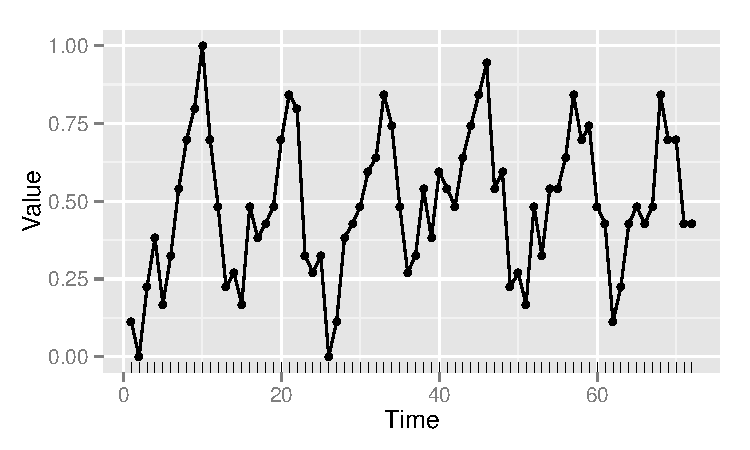
\includegraphics[width=0.48\textwidth]{graph/pipeline-01-regular} 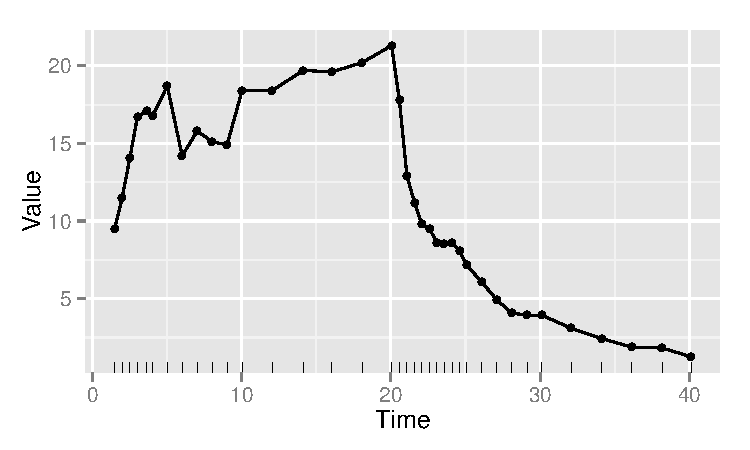
\includegraphics[width=0.48\textwidth]{graph/pipeline-01-irregular}
\end{centering}

\caption{\label{fig:Time-series-plots}Time series plots for regular time spacing
 (left) and irregular time spacing  (right). Tick marks at bottom indicate the time sampling.}
\end{figure}

\subsection{Visualizing time}

Longitudinal data and time series data, although analyzed
very differently, have in common the context of time that
is commonly plotted in similar ways. Below are examples of
common types of temporal displays. Comparing to the time
visualization taxonomy from \citet{aigner2011visualization},
methods here emphasize coordinate arrangement and the
effectivity on information delivery.

Time is conventionally displayed on a horizontal axis of a plot, with many different variations:

\begin{itemize} \itemsep 0in
\item A line graph, the basic building block for temporal data, displays the measured variable on the vertical axis, time horizontally, and consecutive time points are connected with line segments. Figure \ref{fig:Time-series-plots} gives two examples of line graphs, for a single measured variable: (left) a classical time series plot, (right) a profile plot of longitudinal data. When there are many series, for example time series of different stocks or different geographic locations, or many patients, the series may be overlaid on the same plot (Figure \ref{fig:horizontal-axis} row 1 left), or faceted in several blocks (Figure \ref{fig:horizontal-axis} row 1 right).

%\begin{center}
%\begin{figure}[h]
%\begin{centering}
%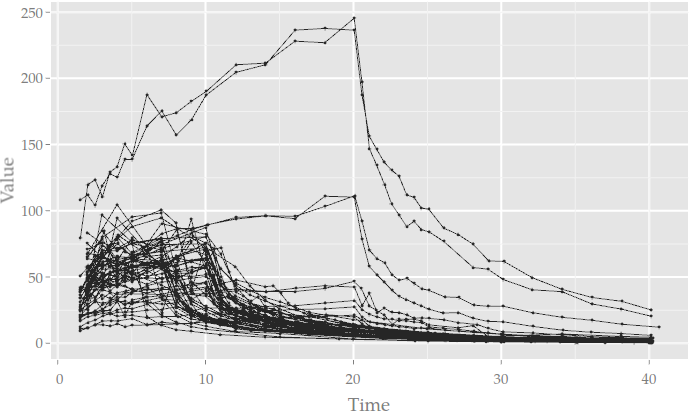
\includegraphics[width=0.6\textwidth]{graph/pipeline-03-2}
%\par\end{centering}
%\caption{\label{fig:Line-graph}Profile plots of longitudinal data for multiple patients. \red{recommend adding examples of small multiples, and other types mentioned here.}}
%\end{figure}
%\par\end{center}

\item Small multiples are used to display multiple series in separate plots (Figure \ref{fig:horizontal-axis} row 2 right). The terminology small multiples was introduced by \citet{tufte1983visual}. A special modification was developed for multiple times series, called sparklines \citet{tufte2006evidence}. Small multiples can also be generated by subsetting based on categorical covariates (e.g. \citet{cleveland1993}).

\item Stacked graphs. Originated by \citeauthor{playfair2005playfair} in
1700's and recently discussed by \citet{byron2008stacked,javed2010graphical,heer2010tour},
a stacked graph draws the time series sequentially, and uses the previous
time series as the baseline for the current series (Figure \ref{fig:horizontal-axis} row 2 left). It is mostly used
for the longitudinal data rather than multivariate time series since
the individuals from the longitudinal data share the same scale.

\item Themeriver and streamgraph. Themeriver is created by \citet{havre2000themeriver},
which is a special case of the stacked graphs, since it moves the
starting baseline from the bottom to the center, and makes the plot
symmetric vertically (Figure \ref{fig:horizontal-axis} row 3 left). Streamgraph is developed later by \citet{byron2008stacked}.
It changed the algorithm to avoid the symmetry which increases the
internal distortion.

\item Horizon graphs. The horizon graph is inspired by two-tone pseudo coloring
\citep{saito2005two} and formally developed at Panopticon Software
\citep{reijner2008development}. Two-tone pseudo coloring is a technique
to visualize the details of multiple time series precisely and effectively.
However, the horizon graph became more popular after mirroring the
lower part of the series and simplifying the color scheme (Figure \ref{fig:horizontal-axis} row 3 right). The horizon
graphs were designed for visualizing the stock prices and economic/financial
data, so the features fit the requirements very well:  (1) The data
have a baseline, which is usually the value at the starting time point.
Then the baseline can be used to mirror the negative part to the positive,
in order to save the graph space, where `negative/positive' means
smaller/greater than the baseline.  (2) The positive and negative performance
should be distinguished, so the horizon graph provides two hues.  (3)
The number of the color bands should be small, usually three color
bands for the positive values and three for the negative. Finding
the band height is easy for the stock prices since they can use 10\%
of the initial value, and in most cases the price will not increase
or decrease for more than 30\%.

\end{itemize}

% When time can be broken into two components it might be displayed
% on both horizontal and vertical axes:
%
% \begin{itemize} \itemsep 0in
% \item A high frequency time series often has hierarchic or nested
% period levels, like year, day, minute, etc. Those levels can
% be placed on horizontal and vertical axes to reveal the periodic
% dependency. For example, \citet{keller1993visual} used days
% and hours on two axes. In these graphs, the measurements of
% the time series are drawn in the grids via aesthetic settings
% like color or size.
%
% \item Calendar heat maps. \citet{van1999cluster} proposed a
% colored calendar visualization  (weeks and days on two axes).
% \texttt{\textbf{d3.js}} \citep{bostock2011d3} applies the calendar
% heat maps and makes it interactive.
% \end{itemize}

Because time in some circumstances can be considered to be cyclical it is sometimes displayed in the polar coordinates:

%As an alternative to the Euclidean coordinates, polar coordinates provide a compact way to visualize the series by rolling the line clockwise or counterclockwise. Any line graphs in Euclidean coordinates can be converted to polar coordinates. Two named graphs to visualize time in polar coordinates are given as follows.

\begin{itemize} \itemsep 0in
\item Nightingale's coxcomb. Florence Nightingale might be the earliest
author of a time series plot in polar coordinates. In the original
plots, two unstacked barcharts were made in polar coordinates. Each
diagram represents for one year. Later, people use the Nightingale's
coxcomb \citep{nightingale1858notes}, also called circular histogram
or rose diagram \citep{nemec1988shape}, to plot the time series with
a regular period like year or day.
\item Spiral graphs. This approach is proposed by \citet{weber2001visualizing}.
It can be seen as a temporal heatmap in polar coordinates. Figure
\ref{fig:polar-axis} (right) shows an example. This approach
is good for seeking the period, but the length for the same time unit
changes over the loops. Besides, spiral graphs would be unhandy for
the short period problems and multiple time series.
\end{itemize}

\begin{center}
\begin{figure}[htp]
\begin{centering}
\begin{tabular}{cc}
(a) & (b) \\
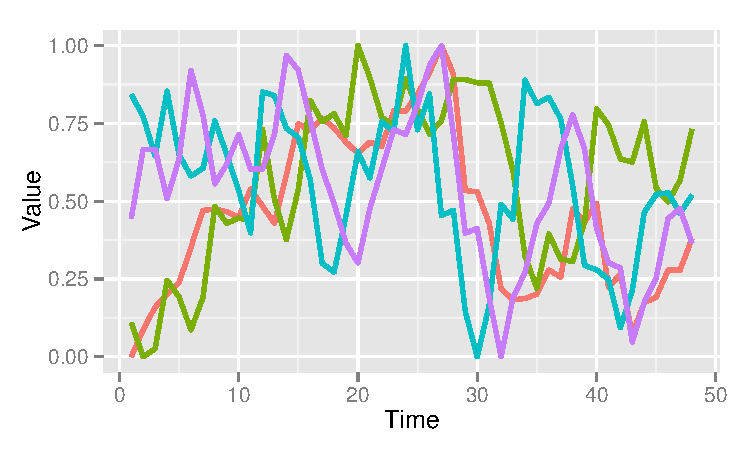
\includegraphics[width=0.48\textwidth]{graph/pipeline-02-linegraph} &
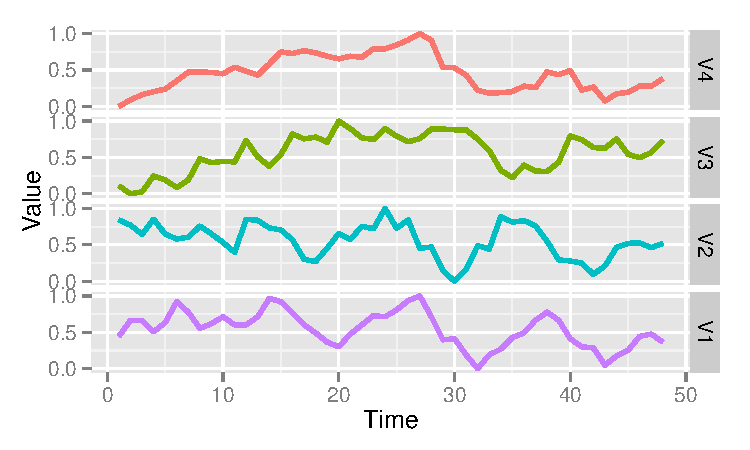
\includegraphics[width=0.48\textwidth]{graph/pipeline-02-multilines}\\
(c) & (d) \\
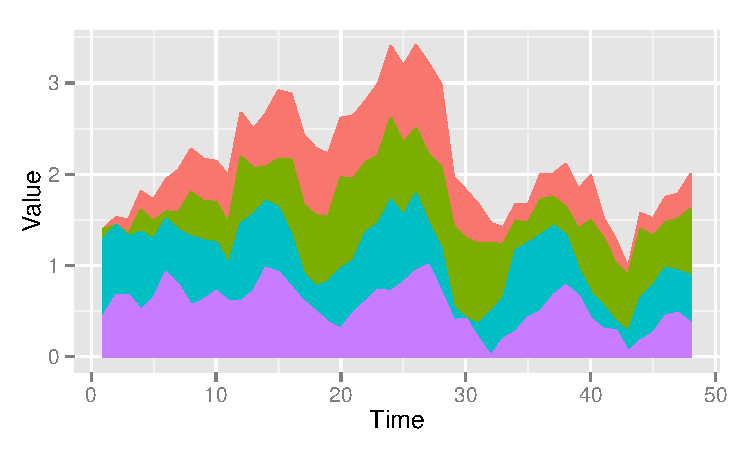
\includegraphics[width=0.48\textwidth]{graph/pipeline-02-stacked} &
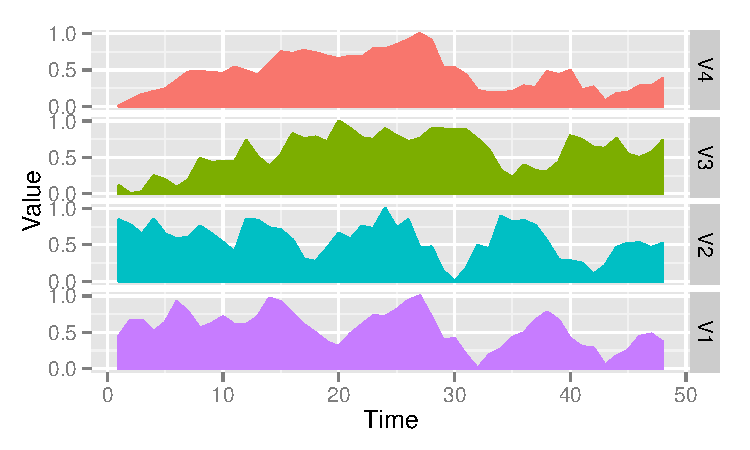
\includegraphics[width=0.48\textwidth]{graph/pipeline-02-smallmultiples}\\
(e) & (f) \\
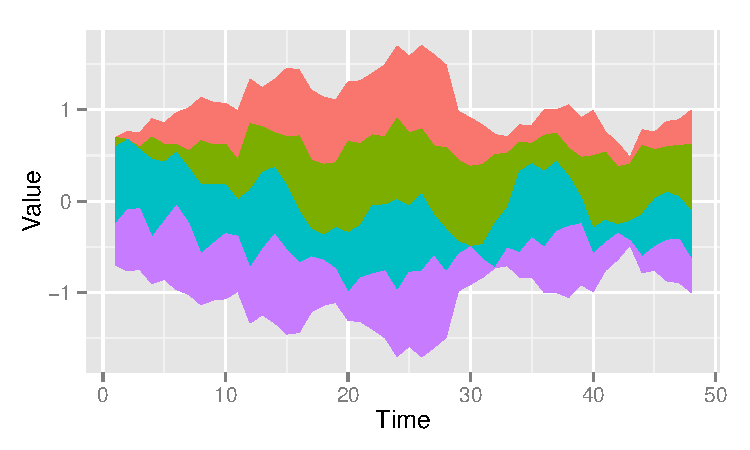
\includegraphics[width=0.48\textwidth]{graph/pipeline-02-themeriver} &
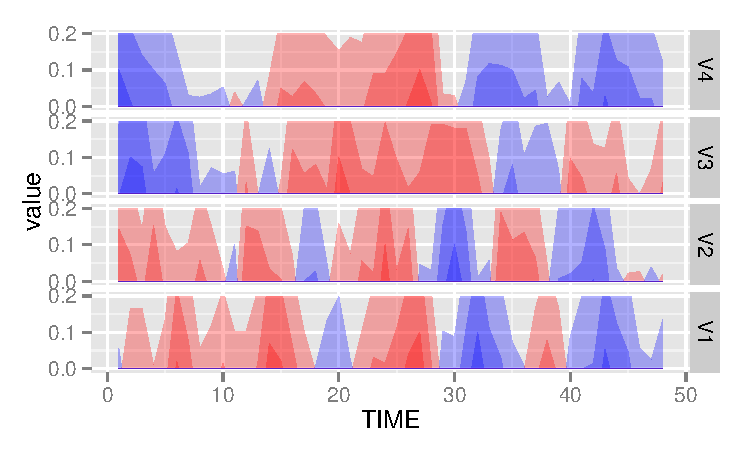
\includegraphics[width=0.48\textwidth]{graph/pipeline-02-horizon}
\end{tabular}
\end{centering}
\caption{\label{fig:horizontal-axis} Six variations of horizontal axis time plots for multivariate
time series: (From top left to bottom right) overlaid line plots, faceted line plots,  stacked graph, faceted area chart, themeriver, horizon graph. Plots in the right column are examples of small multiples. }
\end{figure}
\end{center}

\begin{center}
\begin{figure}[htp]
\begin{centering}
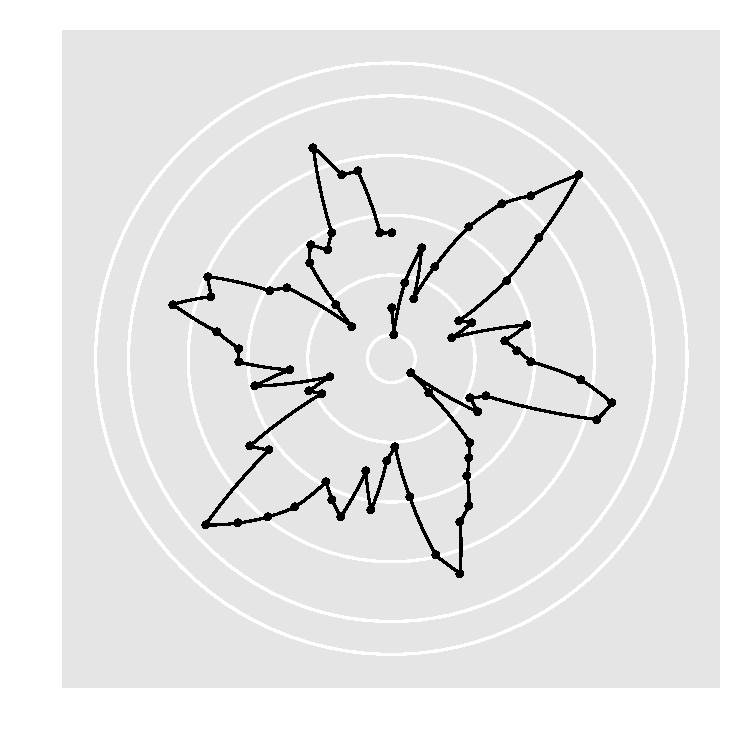
\includegraphics[width=0.32\textwidth]{graph/pipeline-03-polarline}
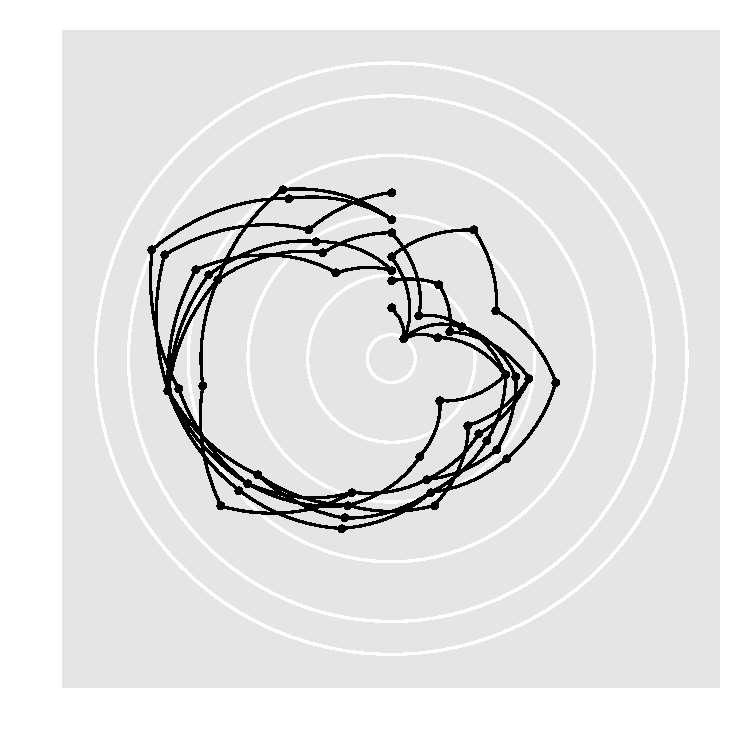
\includegraphics[width=0.32\textwidth]{graph/pipeline-03-polarperiod}
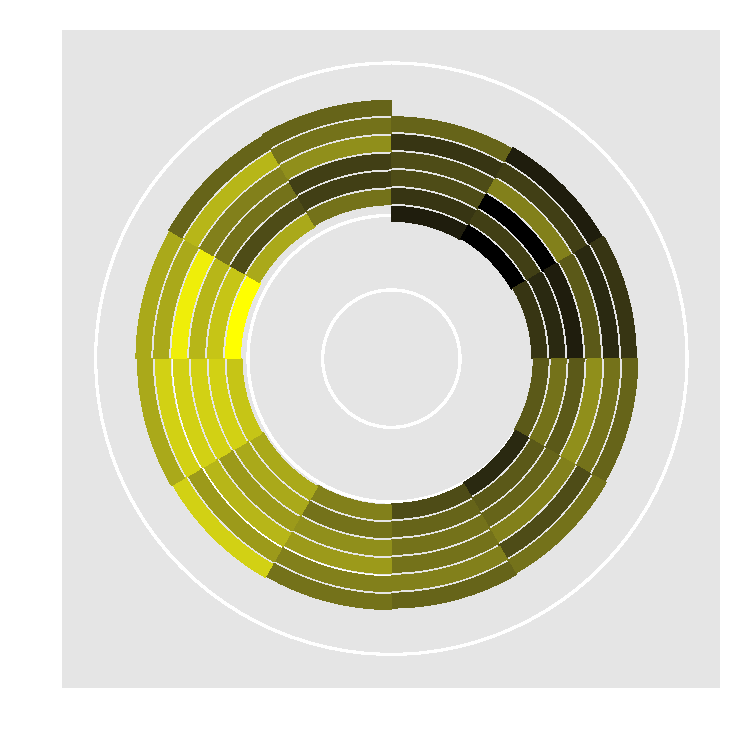
\includegraphics[width=0.32\textwidth]{graph/pipeline-03-spiral}
\end{centering}
\caption{\label{fig:polar-axis}Three types of time series plots
in polar coordinates for the same data as used regularly spaced series shown in Figure
\ref{fig:Time-series-plots}:  direct conversion (left), wrapped by the period (middle), and
spiral graph with the colored grey scale representing the values (right).}
\end{figure}
\end{center}

%\end{enumerate}

\subsection{Interactive graphics\label{sec:interactive-graphics}}

Interactive graphics emphasize the user manipulation of plot elements via input devices like the keyboard and mouse \citep{symanzik2012interactive}. \citet{swayne1999} surveyed the use of the term ``interactive graphics'', which revealed some differences in what people mean when they use the term. They found that most commonly people perceived interactive graphics to mean that a new plot can be recreated quickly from the command line, like base R plots. They suggested using a different term, direct manipulation, to mean directly changing elements of the plot using input devices. However, this term did not gain traction in the community, and we still use interactive graphics. To be clear, we use it here to indicate direct manipulation of plot elements through input actions of mouse or key strokes.

The work described here builds from a history of statistics software systems that support interactive graphics: e.g.
\texttt{\textbf{PRIM-9}}~\citep{fisherkeller1988prim},
\texttt{\textbf{Data Desk}}~\citep{velleman1988datadesk},
\texttt{\textbf{LISP-STAT}}~\citep{tierney1990lisp},
\texttt{\textbf{XGobi}}~\citep{swayne1998xgobi} and
\texttt{\textbf{GGobi}}~\citep{cook2007ggobi},
\texttt{\textbf{MANET}}~\citep{unwin1996manet},
\texttt{\textbf{Mondrian}}~\citep{theus2002mondrian}.
The software \texttt{\textbf{Diamond Fast}}~\citep{unwin1988eyeballing},
\texttt{\textbf{XQz}}~\citep{McDougall1994}, and \texttt{\textbf{Fortune}}~\citep{kotterfortune}  provided tools specifically for exploring time series data.
With the current popularity of R language \citep{Rlanguage}, ideally interactive graphics can
integrate closely and flexibly with statistical modeling. Packages that support this to varying extents are \texttt{\textbf{rggobi}}~\citep{rggobi},
\texttt{\textbf{iplots}}~\citep{iplots},
\texttt{\textbf{rgl}}~\citep{adler2003rgl},
\texttt{\textbf{cranvas}}~\citep{cranvas},
\texttt{\textbf{ggvis}}~\citep{ggvis},
and \texttt{\textbf{animint}}~\citep{animint}.

Of these software, \texttt{\textbf{cranvas}}, which evolved substantially from  \texttt{\textbf{GGobi}}, is the vehicle for the ideas described in this paper.
At its foundation is a data pipeline that channels data to
plot elements, and provides interaction through reactive data
elements, using \texttt{\textbf{plumbr}}~\citep{plumbr2014}. The
graphics are constructed using \texttt{\textbf{Qt}}~\citep{Qt}
that enables flexible plot design and fast rendering for smooth
interaction. \texttt{\textbf{cranvas}} has
many different types of plots and possible interactions.
%Other R packages incorporating interactive graphics have different purposes and strengths. \texttt{\textbf{rgl}} focuses more on 3-d plot rotation. \texttt{\textbf{ggvis}} interactivity is built on top of \texttt{\textbf{shiny}}~\citep{shiny}, and focuses on simple purposes as yet.  \texttt{\textbf{animint}} translates \texttt{\textbf{ggplot2}} to javascript plots.  \texttt{\textbf{iplots}} is the most similar to cranvas. It is built using \texttt{\textbf{Java}}, requires a special GUI, JGR to operate, and provides a smaller set of plot types and interactions.
The design of \texttt{\textbf{cranvas}}, \citet{xie2014reactive} provides single display interactions and the linking between different displays. Single display interactions include brushing, zooming, panning, and querying. Linked brushing can be done between different displays. To integrate temporal displays in this system requires integrating with this setup. % The displays could be either in the same type, or different types, like the scatterplot, histogram, map, etc. These both need to be considered when making interactions on plots for temporal data.

%\red{Shelve these next two paragraphs for now, From another angle, the interactions can be classified by complexity. In a simplest case, the interaction is a one-way, direct manipulation that the user asks the computer to execute directly from the original data and current settings. This type of interactions is usually attached to some action as a handler, which does not require any following command. So nothing needs to be saved from the result. For example, with a graphical user interface (GUI), we can change the graph parameters simply by clicking a button, then the plot will be updated. Another example is querying. \citet{theus2011interactive} gave a well description on how to query the information, where the ``command'' is pausing the mouse icon on an object.

%Under some complicated situations, a single manipulation cannot give a satisfactory result. For example, to explore the features of a set of variables conditional on another set of variables, brushing on a fixed area is not enough. We may need to move the brush from one side to the other side of the conditional variables, to detect the trend of interest. And if needed, we may change the brush size, or select the union of some separate areas. It is usually a series of continual manipulations, based on the instant computer output. Hence this bidirectional complex type of interactions will requires the accessibility to the result at any time, to prepare for the next command.

%This characterisitic of the complex interactions brings at least two issues: rewritability of the result storage, and accessibility from different function environments to the result. \citet{xie2014reactive} solved the second issue based on the design of \texttt{\textbf{cranvas}}.

%This paper is organized in the following way.
The next section describes the building blocks for temporal displays, which is followed by a taxonomy of interactive tasks that is desirable to use for exploration (Section \ref{sec:Design-of-interactions}). How to realize the interactions is described in Section \ref{sec:Pipeline}. Linking between temporal data displays and other plots is described in Section \ref{sec:Linking}.


\section{Layering to create a plot\label{sec:graph-layers}}

For interactive graphics, layering up the plot to enable
different interactions can be useful, and efficient for
large data. The base layer is typically the plot of all
of the data. An overlay of a brush layer, where only
elements actively being colored are displayed, can provide
the efficiency of faster rendering. A brush layer is
common to all displays because brushing is a basic function
for interactive graphics. Background layers like an axis
layer or grid layer are common too, but are not necessary
in displays like maps. \texttt{\textbf{cranvas}} provides
some specific layers for different plot types. For instance,
a \texttt{\textbf{cranvas}} map composes of four layers:
polygon, googlemaps, path, and point layer.

%Table \ref{tab:Layers} lists the layers of common plot types in \texttt{\textbf{cranvas}}.
%we can different layers are desired as the plot regions by different interactions. Usually there are many layers for an interactive graph, because a complex interaction can be then decomposed into small simple tasks on different layers. One layer is often designed for only one graph element, like the title layer, x-axis layer, or brush layer. Based on the characteristics of the graph elements, different painting functions are used to make the plotting fast for layers. When one layer changes, the irrelevant layers will remain the same.


% \begin{center}
% \begin{table}[h]
% \begin{center}
% \begin{tabular}{c|l|l}
% \hline
%   & scatterplot & point\tabularnewline
% \cline{2-3}
% display specific & histogram & bar, cue\tabularnewline
% \cline{2-3}
%  & map & polygon, googlemaps, path, point\tabularnewline
% \cline{2-3}
%  & time plot & point, line, area, stats\tabularnewline
% \hline
% common & required & brush, identify, keys\tabularnewline
% \cline{2-3}
%  & optional & grid, $x$-axis, $y$-axis, $x$-label, $y$-label, title \tabularnewline
% \hline
% \end{tabular}
% \end{center}
%
% \caption{\label{tab:Layers}Examples from \texttt{\textbf{cranvas}}
% of layers used in constructing plots. Some are common to all plots,
% and each plot has some layers that are unique. The ``keys'' layer
% listens for key strokes that change interaction modes. The ``cue''
% layer on the histogram contains listeners and handles for dragging
% to change the binwidth interactively.}
% \end{table}
%
% \end{center}


%\begin{center}
%\begin{figure}[h]
%\begin{centering}
%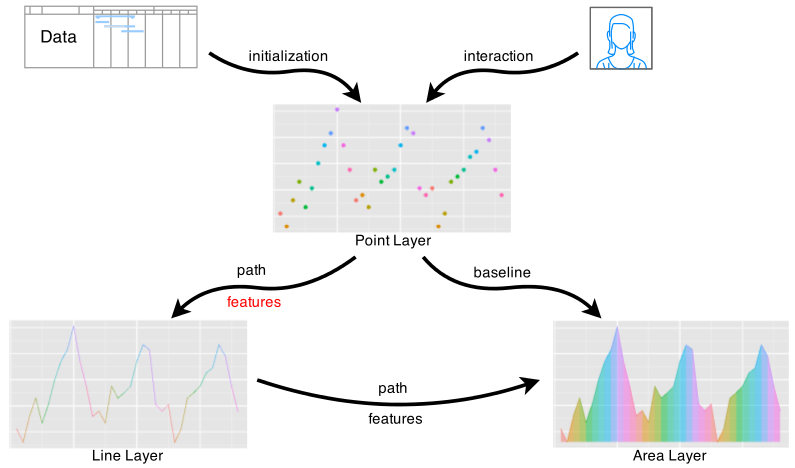
\includegraphics[width=0.8\textwidth]{graph/pipeline-12-threelayers}
%\par\end{centering}

%\caption{\label{fig:layer-system}The point layer is the center of the system that receives the data and interactions at first. Then the line and area layers adopt the current position and features from the point layer. The color of the lines is determined by the color of the first point in the pair defining the line segment. The color of the polygon is driven by the color of the line segment.}
%\end{figure}

%\par\end{center}


For temporal data displays, there are three basic layers: point, line, and area. The coordinates of the points are initially calculated from the data, and interactions may change the locations of the points in the display. The line layer connects the current positions of the points, so it requires the order, or, path information to know how to make the connections. The area layer shades the area under the line by constructing a baseline, matching the minimum data values, which enables closing the series to create a set of polygons.  %Figure \ref{fig:layer-system} shows the relationship among three layers.
Each of these layers can take different interactions, and some care needs to be taken in realizing the effect on the different layers.

%\begin{enumerate} \itemsep 0in
%\item Transmission of the brushing information.
The point attributes, selected, color, size, or visibility, are generated for each observation when creating the plumbr mutaframe. The base element for the temporal plots are the points, and in \texttt{\textbf{cranvas}} brushing changes the attribute of each point in the mutaframe -- essentially, points are brushed. The number of lines is one less than the number of points, and line color follows the first point in the defining pair. The number of polygons for the area display is the same as the number of lines, so color follows lines directly to polygons. The additional construction points of the area layer are only used in the area layer, and do not have independent attributes. This affects brushing behavior which is discussed later.

%However, translating this to edges is not simply defined because one edge connects two points, $\# points=\# edges+1$, and for a multivariate time plot with $n$ series,  $\# points=\#edges+n.$ In the area layer, each polygon is defined by a number of edges, i.e., $\#polygons=\#edges$. %As shown in Figure \ref{fig:layer-system},  The color of lines follows from the color of the first point of the line segment, and the color of polygons descends from the lines.

%\begin{center}
%\begin{figure}[htp]
%\begin{centering}
%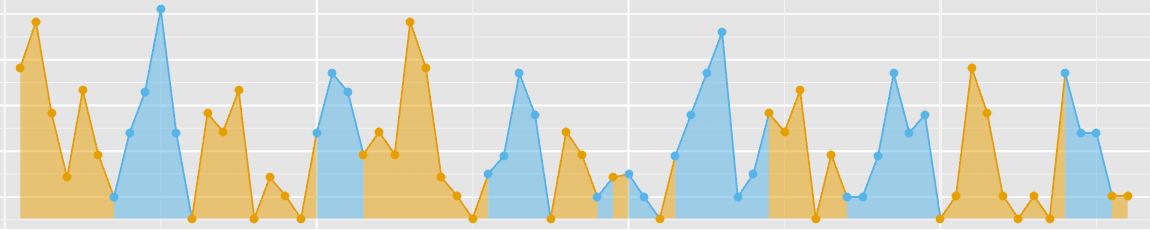
\includegraphics[width=0.4\textwidth]{graph/pipeline-13-layer-features}
%\par\end{centering}
%\caption{\label{fig:features}Illustration of the coloring logic for the different layers -- everything is driven by the point layer. Each point here has a different color. The color of the lines is determined by the color of the first point in the pair defining the line segment. The color of the polygon is driven by the color of the line segment.}
%\end{figure}
%\par\end{center}

% brushing Now the problem is, how to get the painting features for each edge and polygon? It is easy to answer the question when the features of points are identical. But when they are varied, we have to skip the features of $n$ points for $n$ lines by Equation  (\ref{eq:points_edges}). Then how to choose the $n$ points? One possible but not perfect solution is the first or last point of a line.%, like shown in Figure \ref{fig:features}. A smoother method should be considered for the edges and polygons that connect two points with different features. To make it convenient for the interactions, the method should be simple and avoid involving new coordinates.

%\item
%The area layer typically will need additional construction points, which are considered to be part of the area layer, but not the point layer. The point layer needs the $x/y$ coordinates, while the line layer needs the $x/y$ coordinates in order and in groups. But the area layer incorporates a baseline, which is generated by calculating the minimum of the values on the variable. When the $y$-coordinates change, as happens when facetting, the baseline needs to be updated instantly. The additional information challenges the linking system, and some details are discussed in Section \ref{sub:Linking-of-the-addition}.

% \begin{center}
% \begin{table}[htp]
% \begin{centering}
% {\small{}}%
% \begin{tabular}{ccc}
% {Point layer} & {Line layer} & {Area layer}\tabularnewline\tabularnewline
% {\small{}}%
% \begin{tabular}{|c|c|l|}
% \hline
% {\small{$x$}} & {\small{$y$}} & {\small{color}}\tabularnewline
% \hline
% {\small{1}} & {\small{3}} & {\small{peach}}\tabularnewline
% {\small{2}} & {\small{5}} & {\small{olive}}\tabularnewline
% {\small{3}} & {\small{2}} & {\small{cyan}}\tabularnewline
% {\small{4}} & {\small{4}} & {\small{purple}}\tabularnewline
% {\small{5}} & {\small{3}} & {\small{peach}}\tabularnewline
% \hline
% \end{tabular} & {\small{}}%
% \begin{tabular}{|cc|cc|l|}
% \hline
% {\small{$x_1$}} & {\small{$x_2$}} & {\small{$y_1$}} & {\small{$y_2$}} & {\small{color}}\tabularnewline
% \hline
% {\small{1}} & {\small{2}} & {\small{3}} & {\small{5}} & {\small{peach}}\tabularnewline
% {\small{2}} & {\small{3}} & {\small{5}} & {\small{2}} & {\small{olive}}\tabularnewline
% {\small{3}} & {\small{4}} & {\small{2}} & {\small{4}} & {\small{cyan}}\tabularnewline
% {\small{4}} & {\small{5}} & {\small{4}} & {\small{3}} & {\small{purple}}\tabularnewline
% \hline
% \multicolumn{1}{c}{} & \multicolumn{1}{c}{} &  & \multicolumn{1}{c}{} & \multicolumn{1}{c}{}\tabularnewline
% \end{tabular} & {\small{}}%
% \begin{tabular}{|cccc|cccc|l|}
% \hline
% {\small{$x_1$}} & {\small{$x_2$}} & {\small{$x_3$}} & {\small{$x_4$}} & {\small{$y_1$}} & {\small{$y_2$}} & {\small{$y_3$}} & {\small{$y_4$}} & {\small{color}}\tabularnewline
% \hline
% {\small{1}} & {\small{2}} & {\small{2}} & {\small{1}} & {\small{3}} & {\small{5}} & {\small{1}} & {\small{1}} & {\small{peach}}\tabularnewline
% {\small{2}} & {\small{3}} & {\small{3}} & {\small{2}} & {\small{5}} & {\small{2}} & {\small{1}} & {\small{1}} & {\small{olive}}\tabularnewline
% {\small{3}} & {\small{4}} & {\small{4}} & {\small{3}} & {\small{2}} & {\small{4}} & {\small{1}} & {\small{1}} & {\small{cyan}}\tabularnewline
% {\small{4}} & {\small{5}} & {\small{5}} & {\small{4}} & {\small{4}} & {\small{3}} & {\small{1}} & {\small{1}} & {\small{purple}}\tabularnewline
% \hline
% \multicolumn{1}{c}{} &  &  & \multicolumn{1}{c}{} &  &  &  & \multicolumn{1}{c}{} & \multicolumn{1}{c}{}\tabularnewline
% \end{tabular}\tabularnewline
% \end{tabular}
% \par\end{centering}{\small \par}
%
% \caption{\label{tab:coordinates-for-layers}Data to generate three layers for Figure \ref{fig:features}. The data for point layer is in the same structure as the original time series. In the line layer, coordinates for both sides of four edges are generated from the point data. More structural points are needed for the area layer to form the baseline -- here a $y$-value of 1 is chosen as the baseline. The $x$/$y$ coordinates for four vertexes in each polygon are given, in which the first two columns for both $x$ and $y$ are adopted from the line layer.}
% \end{table}
% \par\end{center}

%\end{enumerate}


\section{A taxonomy of interactions for temporal data displays\label{sec:Design-of-interactions}}

\citet{wills2012visualizing} summarizes
the interactivity for temporal displays as changes to parameters or data. Data is mapped into coordinates in the plot. Parameters can be considered to be attributes like color, labels, geometric elements, facet, or they can be considered to be aspects used to get the data into the plot like transformations, binning, dimension reductions or scales. Changes to the data or parameters provoke changes to the plots.

Parameters can often be attached to graphical user interface (GUI) items like sliders, that can generate the change in the plot. But more generally, interactions happen by direct action on the plot. For example, in brushing, the user selects elements like points in the plots. The software needs to locate these items in the data, update the attributes of these selected points, and broadcast these changes to other plots.

%On one hand, the parameters are modified for the purpose of changing the element, aesthetic, coordinate, statistic, scale, facet, or transform, while the data remain the same. On the other hand, to brush, link, or drill-down (zoom-in), the data are modified -- not necessarily the positional information, but also the augmented variables used in the display. However, some of the ideas for the parameters are conceptual and there is no software to integrate them all.

%In reality, the interactions like brushing, selection, linking, zooming, panning, and querying, were already embedded in some interactive graphics software. The software mentioned in Section \ref{sec:interactive-graphics} for time series and longitudinal data used some or all of the interactions.

%Within the realized interactions mentioned above, all but querying belong to the complex type of interactions, based on the discussion in Section \ref{sec:interactive-graphics}. For more explanation, brushing requires the knowledge of the current brush location, and returns the corresponding brushed points. Selection hears from the selection methods, the current selected points, and the cursor location, to return the new selected points. Linking transmits the brushed status from one graph object to another. Zooming and panning uses the current cursor location and zooming range to anchor the new range. All of these returned objects or status should be saved for future use. Hence, the strength of the above software is to support the instantly data exploration conveniently, compared to other interactive tools like GUI.

Some interactions, like brushing, selection, linking, zooming, panning, and querying, are universal for all plot types. Temporal and longitudinal data solicit special interactions to explore aspects of temporal dependence and trend. % In this section we introduce the design of the interactions % and discuss the the interactivity issues.
\citet{Buja1996} describe a taxonomy of interactive tasks for multivariate data. Here we describe a taxonomy of tasks for temporal data, that enable exploration of different components of time series and longitudinal data:

%\subsection{A taxonomy of tasks\label{sub:Special-interactions}}

\begin{itemize} \itemsep 0in
\item Wrapping: In the $x$-direction explores seasonality and
  temporal dependence.  In the $y$-direction it is done to compare
  magnitude of peaks and dips. It is easiest to explain $x$-wrapping:
  the series is cut at a fixed-length interval, the part of the series
  that extends beyond this interval is re-drawn from the initial
  point. This will change the $x$-coordinates of the data. The main
  purpose of $x$-wrapping is to explore the regularity of the
  periodicity. Some series that look to follow a regular period can be
  quickly revealed to have irregularities. The classical example is
  the lynx trappings data for 1821\textendash{}1934 in the MacKenzie
  River District of North-West Canada\citep{campbell1977survey}, which
  looks periodic (Figure \ref{fig:x-wrapping}). The wrapping shows
  that the period is not quite regular, matching one peak off-sets
  other peaks, and the period varies between 9-11 years. It is also
  possible to see that the increases are slower than the drops, that
  the population builds up and tends to plummet. To model this data
  well requires one also knows the snowshoe hare population. Figure
  \ref{fig:y-wrapping} gives an example of the $y$-wrapping. It
  shows another classical example: quarterly pig production measured
  by four variables, herd size, production, profit and gilts, from
  1967-1978 in United Kingdom \citep{andrews1985data}. The $y$-wrapping
  induces something that might be considered a temporal boxplot, where
  density produced from overlaying the wrapped peaks emphasizes long
  runs of ups, or periodic ups.
 %Wrapping cuts the series by a fixed-length interval in the horizontal or vertical direction, and shifts the right/top pieces to the left/bottom. It could change the $x$- / $y$- coordinates of the data. There are two reasons for wrapping. The first one is to compare the periods, or to find the period for the data that is potentially periodical. Also the periodic variation could be explored \citep{mcdonald1986periodic}. For this purpose we suggest to wrap the series horizontally. % Figure \ref{fig:faceting-period} (left to center) gives an % example of horizontal wrapping with a known period. Figure \ref{fig:x-wrapping} shows an example of wrapping process with an unknown period.
%The second reason is to cut the temporal and longitudinal data into parts for a better aspect ratio which will increase the effectiveness of data display \citep{cleveland1987graphical}, and then reveal more details. When the time series is long, to keep a proper aspect ratio is not always workable, due to the the limit of the screen width. Two possible solutions are:  (1) if the series is periodical, then wrap it horizontally by the period, as Figure %\ref{fig:faceting-period} \ref{fig:x-wrapping},  (2) Wrap the series vertically, especially when multiple series are faceted.
%Figure \ref{fig:y-wrapping} gives an example of the y-vertical wrapping for quarterly pig production from 1967-1978 in United Kingdom \citep{andrews1985data}. The four variables are HERDSZ: actual breeding herd size, PRODUCTION: number of clean pig meat slaughtered, PROFIT: ratio of all-pig price to all fattener feed price, GILTS: number of sows in pig for the first time. In the top panel we see some overall pattern but it is hard to compare two values from the first quarter and last quarter of a line. In the bottom panel the series are wrapped in an area plot. The darkness of the colors indicates the magnitude of the series values, and the color bands make the comparison within or between the series much easier.
\item Faceting: This creates small multiples to organize and examine across structural data components. These components might be a period such as year, or month, or variables when multiple are measured at the same time points, or in longitudinal data these might be individuals. In the interactive setting these components can be used to slowly pull overlaid series apart, a process that might be more revealing that disjointly laying out each in a static plot. Figure \ref{fig:faceting-var-ind} illustrates sequential faceting on two variables and three individuals. The order of these operations changes the final result, and changes which comparison is primary and which secondary. Figure \ref{fig:faceting-examples} gives two more examples, by a grid of spatial locations, and by covariates, respectively. Watch the videos to see how these are achieved interactively. There is also another video at \url{https://vimeo.com/112505175} shows faceting on period for a time series with a regular period of every 12 observations.

%Sometimes we care about some objects or time intervals more than others, for instance, the patients under a special treatment, or the climate observations in a year when the earthquakes frequently happened. In other cases with many variables, we may have questions like whether the variables share the same period? Do the peaks and valleys match with each other? To explore the data with these questions, we need to compare multiple time series.

%In a static graph, several aesthetic methods can be used to distinguish and compare multiple lines, like the color, size, or line type. However, the aesthetic methods are not encouraged for a relatively large number of lines, say, more than 10 lines. This is because the difference of colors, sizes, or line types between adjacent lines could be too weak to tell. Hence, faceting is considered as a technique to reduce the number of lines displayed in the same plotting region. Users can compare within and between facet regions easily when the aspect ratio keeps well.

%There are three possible conditions to facet on: variable, individual (for the longitudinal data), or period. Those faceting methods change the coordinates of the points, and then the baselines of the area layer. Figure \ref{fig:faceting-var-ind} gives an example for faceting on two variables and three individuals. Design of the faceting interaction should make the switching among five panels done on-the-fly.
% Figure \ref{fig:faceting-period} explains why and shows how to facet on period.

%Faceting by individual sometimes extends to much more complex situations, because individuals can be grouped under different combinations of categorical variables, not only the individual IDs. Both horizontal and vertical directions will be needed to facet, and in each direction, more than one variable may be utilized to facet. For example, Figure \ref{fig:faceting-2ind} shows faceting on individual by two independent groups  (longitude and latitude). Figure \ref{fig:faceting-4ind} shows faceting by four categorical variables, two in the horizontal direction and two in the vertical direction.

%It is apparent that faceting by either variable, individual or both helps to find the similar or unusual temporal pattern among variables and individuals. To realize this functionality we use the variables as the $y$ input, and specify the variable name that indicates the individuals or groups. Faceting on period is similar as faceting on individual -- in both ways the observations are grouped by a variable indicator and the points within group are connected. But the faceting-on-period interaction can not be substituted by faceting on individual, because faceting on period needs to re-index the time points. Figure \ref{fig:x-wrapping} (e) shows faceting on an irregular period. The video at \url{https://vimeo.com/112505175} illustrates an example of faceting on period for a time series with a regular period of every 12 observations.

% If we treat the period as the individual, then each period has one
% line of the same length, so we can plot them together and use the
% individual faceting method to separate the lines. But the answer
% is no. Two things are ignored in the idea. First, it assumes that
% the period exists as a variable in the data, like the year for
% monthly data. Second, it assumes that the time indexes for each
% period are already the same. For example, in Figure \ref{fig:faceting-period} (left),
% the time indexes for the original series are from 1-72. The indexes
% for the six periods are 1-12, 13-24, 25-36, 37-48, 49-60, 61-72,
% respectively. If we facet the period as faceting by individual,
% then the six lines are separated vertically and also horizontally,
% which is different from Figure \ref{fig:faceting-period} (right).

% \begin{center}
% \begin{figure}[htp]
% \begin{centering}
% 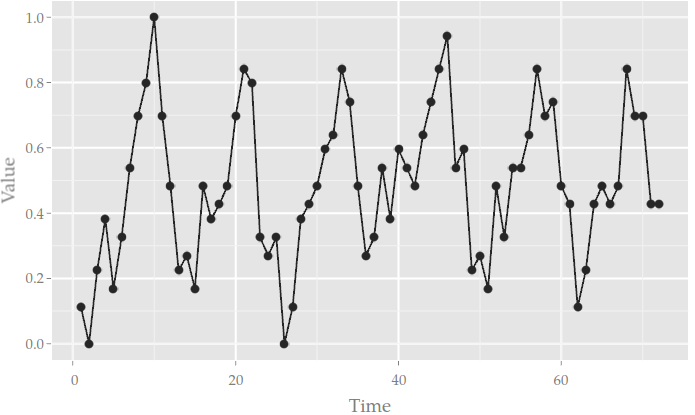
\includegraphics[width=0.32\textwidth]{graph/pipeline-01-1}
% 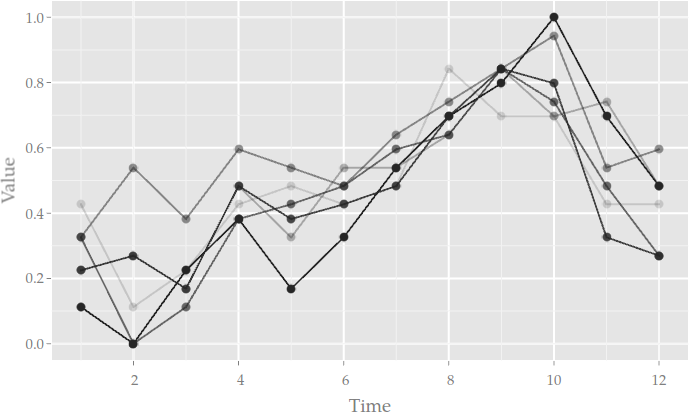
\includegraphics[width=0.32\textwidth]{graph/pipeline-15-5}
% 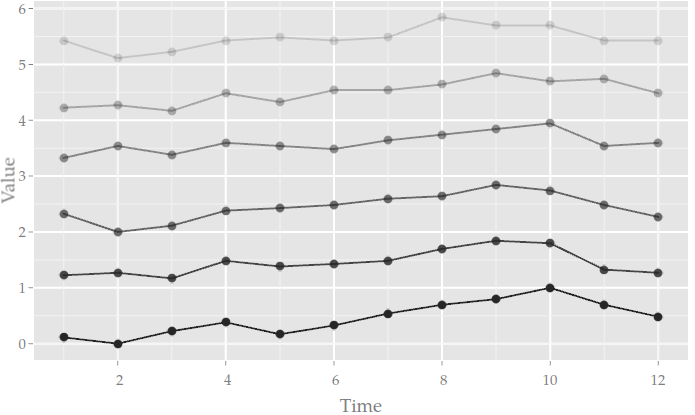
\includegraphics[width=0.32\textwidth]{graph/pipeline-15-3}
% \par\end{centering}
% \caption{\label{fig:faceting-period}An example of faceting on period
% for a time series with a period of every 12 observations. The left
% panel is the original series, the center and right panels show the
% periods before and after faceting. From the left to center, the
% wrapping interaction is used.}
% \end{figure}
% \par\end{center}


\item Mirroring: This splits the series vertically at a given value,
  and reflects the bottom half across this axis. With additional
  wrapping, the result is called a horizon graph, and it is used to
compare the magnitude of peaks and troughs, particularly for binary
phenomena like gains and losses. The $y$-coordinates of the data are
modified by this interaction. The choice of split value are typically
mean, median, midpoint of the range, or in economic data the initial
series value. Figure \ref{fig:x-wrapping} (f) and (g) shows mirroring
of the lynx trappings data with the mean divider. We can see the peaks
are sharp and irregular and the valleys are smooth and regular.
%s that  helps to compare the extreme values of the two sides, save more room for the main body, and provide a better display for the series with  binary features like loss and earning. It dichotomizes the series by  a horizontal divider and reflects the bottom area up to the divider  with a change of the color scheme. The $y$-coordinates of the data  are modified by this interaction.
%However, two issues raise up during the mirroring process:  (1) how to choose the horizontal divider -- midpoint of the range, mean of the series, or the initial value? For the financial related data, the starting value is preferred, like the price when entering the market. But for other types of time series, the choice would depend on the research interest.  (2) when an edge crosses the divider, the intersection will be a new data point to the line and need to be recorded. The new data points could make problems, especially when other interactions are added on the mirrored graph, like wrapping or linking. Section \ref{sub:Linking-of-the-addition} introduces the problems from the additional data in linking.
% \begin{center}
% \begin{figure}[htp]
% \begin{centering}
% 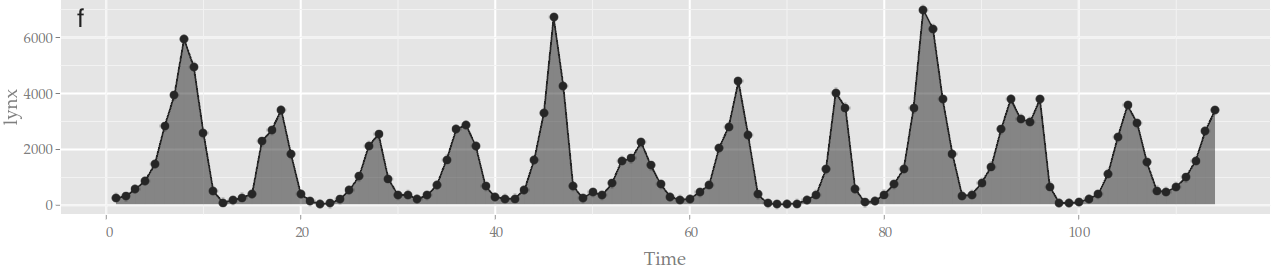
\includegraphics[width=0.98\textwidth]{graph/pipeline-18-original}
% \par\end{centering}
% \begin{centering}
% 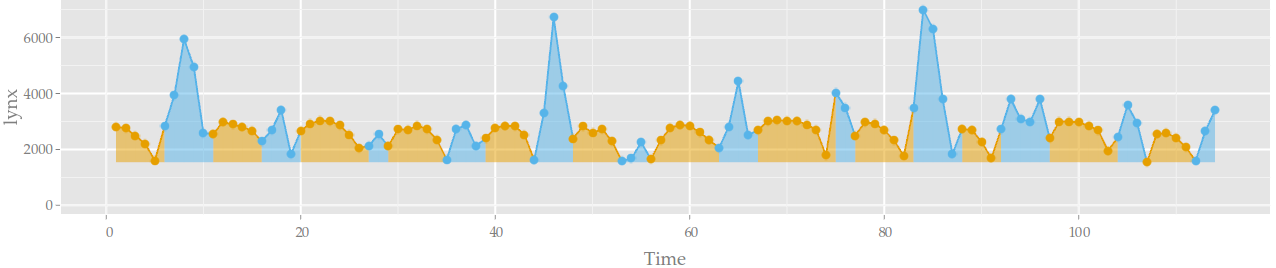
\includegraphics[width=0.98\textwidth]{graph/pipeline-18-mirrored}
% \par\end{centering}
% \caption{\label{fig:mirroring}Top: area plot for the lynx trappings data.
% Bottom: mirroring by the mean. Two colors are assigned to the upper
% and lower part: blue are the values above the mean, yellow below the
% mean. The video at \url{https://vimeo.com/112432400} shows these interactions.}
% \end{figure}
% \par\end{center}

\item Shifting: A series can be grabbed and shifted against another series. This is a more tangible operation than wrapping in order to compare periodicity and temporal dependence. Figure \ref{fig:x-shifting} shows three series that have been picked up and shifted together against the other three series to match peaks.

%exploring dependence between series. When there are multiple series, we may consider to shift one or more series horizontally to match with others for some reason, like the starting time of the series is not the same, or one variable is leading another. This interaction will modify the $x$-coordinates for the selected series.

%Figure \ref{fig:x-shifting} shows how shifting reveals the leading pattern. From the left panel we see variable B  (blue lines) has all its pumps later than variable A  (red lines), but we are not sure if the lag is fixed or varied. So we can shift variable A to the right by four time points and get the right panel. The peaks and valleys match well for the two variables, which confirms the guess of leading pattern.

\item Switching: At any time it should be possible to switch between line and area displays. Line plots are efficient but filling the area under the curve can give a stronger sense of the patterns in the series, especially when trying to compare multiple series.   The video at \url{https://vimeo.com/112530645} demonstrates switching.

%Starting from the basic demand, the interactive time plots should support the switch between the line and area layers, as the line and area plots have their own pluses and minuses. The line plots are concise when comparing the series in the same scales, in contrast the area plots make the space noisy with the overlapping area. In some other cases like the small multiples, the area plots are better because when the baselines are not of the same height, the area makes the understanding and comparison more accurate between values from different series. The video at \url{https://vimeo.com/112530645} demonstrates two situations when the line plot or area plot is preferred.

% As shown in Figure \ref{fig:switching-layers} (1), the area draws much
% attention but not necessary. In Figure \ref{fig:switching-layers} (2),
% the line plot does not deliver the information as clearly as the area
% plot, on the overall high values of series B1 and low values of series A1.

% Switching between the layers does not change the data  (just need to
% add the baselines), but the following interactions will require for
% some data modification.

% \begin{figure}[htp]
% \begin{centering}
% \begin{tabular}{cc}
% \multicolumn{2}{c}{{\scriptsize{ (1) Line plot is better than the area plot.}}}\tabularnewline
% 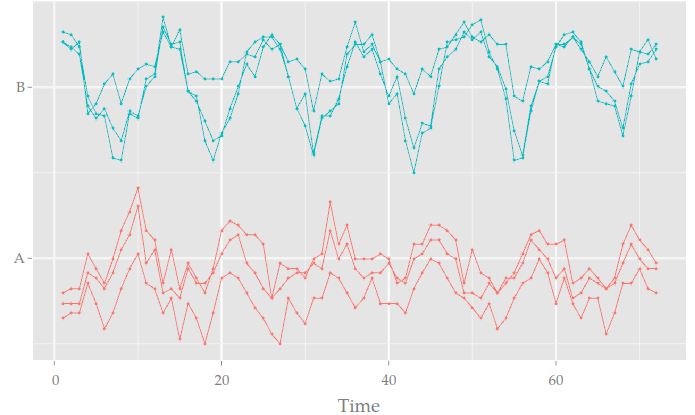
\includegraphics[width=0.48\textwidth]{graph/pipeline-14-6} & 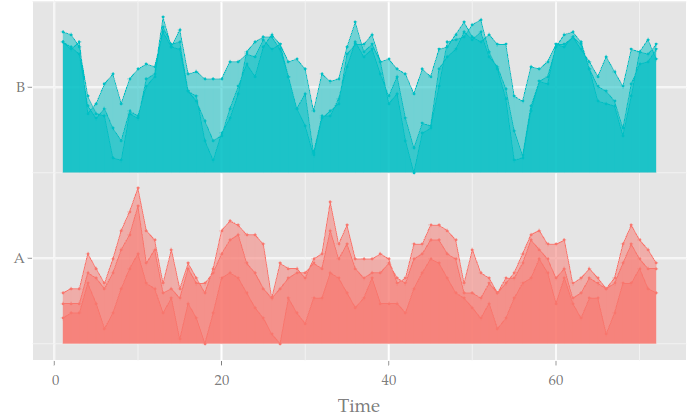
\includegraphics[width=0.48\textwidth]{graph/pipeline-14-8}\tabularnewline
%  & \tabularnewline
% \multicolumn{2}{c}{{\scriptsize{ (2) Area plot is better than the line plot.}}}\tabularnewline
% 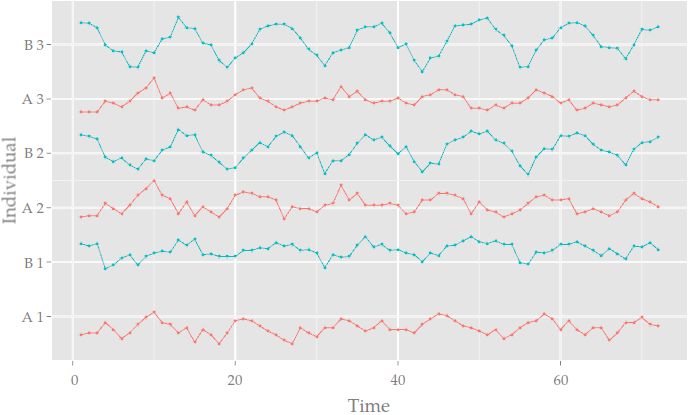
\includegraphics[width=0.48\textwidth]{graph/pipeline-14-7} & 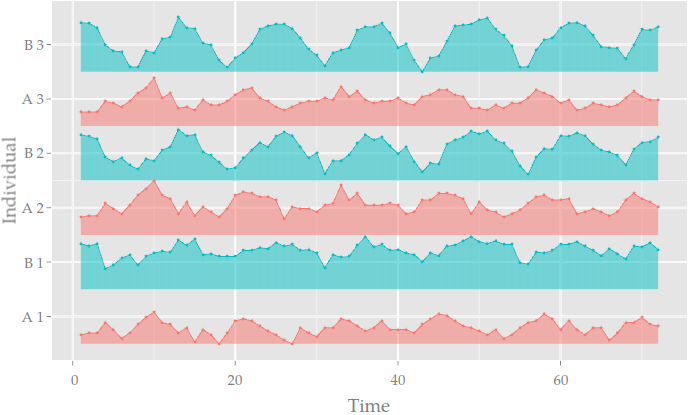
\includegraphics[width=0.48\textwidth]{graph/pipeline-14-9}\tabularnewline
% \end{tabular}
% \par\end{centering}
% \caption{\label{fig:switching-layers}Switching between the line plot and the
% area plot. The line plot is preferred in the first row for the compact
% design without losing information. The area plot is preferred in the
% second row for the easier comparison among values in different lines. Swithcing is illustrated in \url{https://vimeo.com/112530645}. }
% \end{figure}

\end{itemize}

\begin{figure}[htp]
\begin{center}
\begin{tabular}{cc}
%\multicolumn{2}{c}{\small{(a)}}\\
\multicolumn{2}{c}{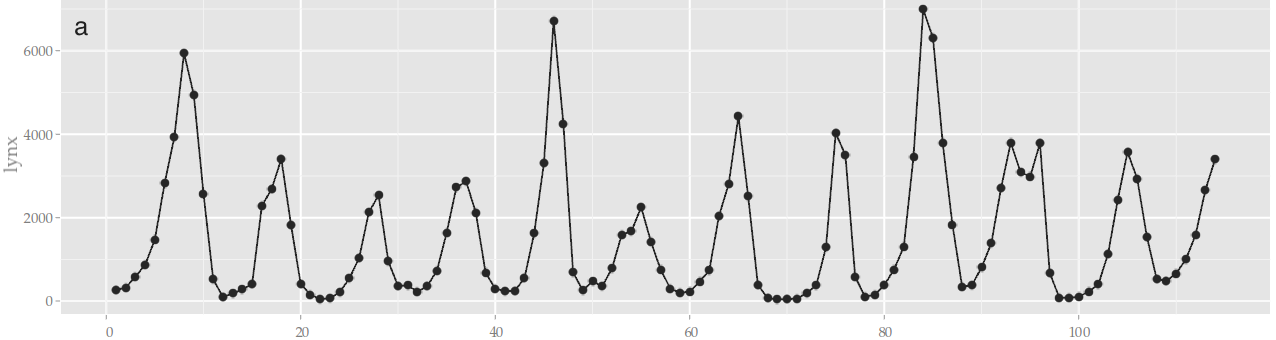
\includegraphics[width=0.8\textwidth]{graph/pipeline-16-original}}\\
%\small{(b)} & \small{(c)} \\
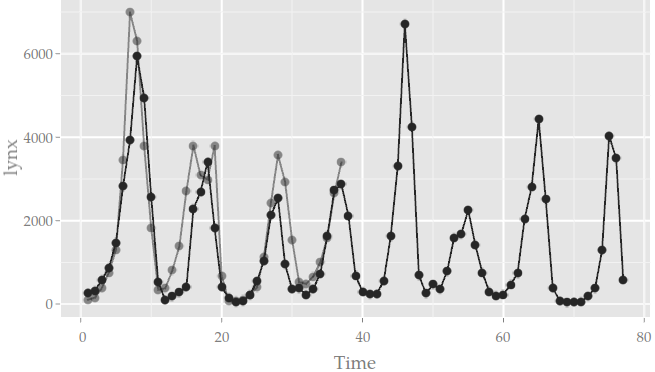
\includegraphics[width=0.4\textwidth]{graph/pipeline-16-1} &
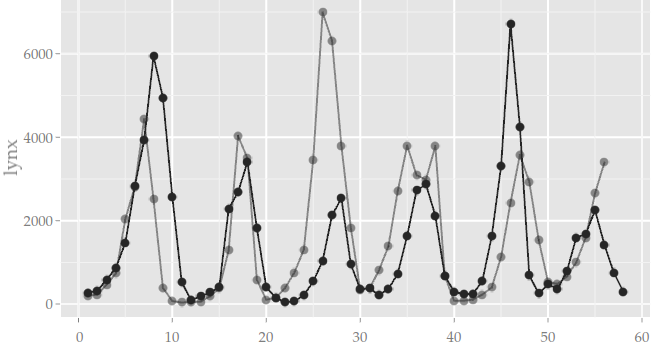
\includegraphics[width=0.4\textwidth]{graph/pipeline-16-2} \\
%\small{(d)} & \small{(e)} \\
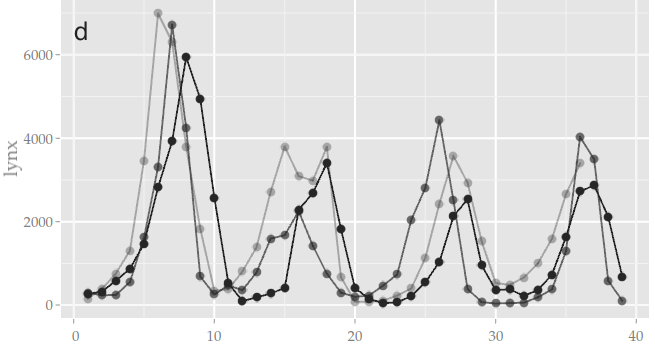
\includegraphics[width=0.4\textwidth]{graph/pipeline-16-xwrap} &
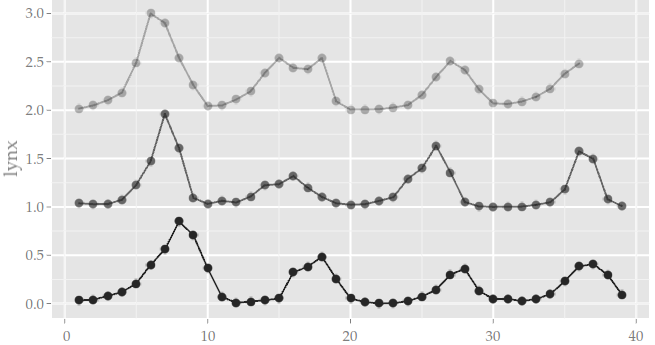
\includegraphics[width=0.4\textwidth]{graph/pipeline-16-xwrap-facet} \\
%\multicolumn{2}{c}{\small{(f)}} \\
\multicolumn{2}{c}{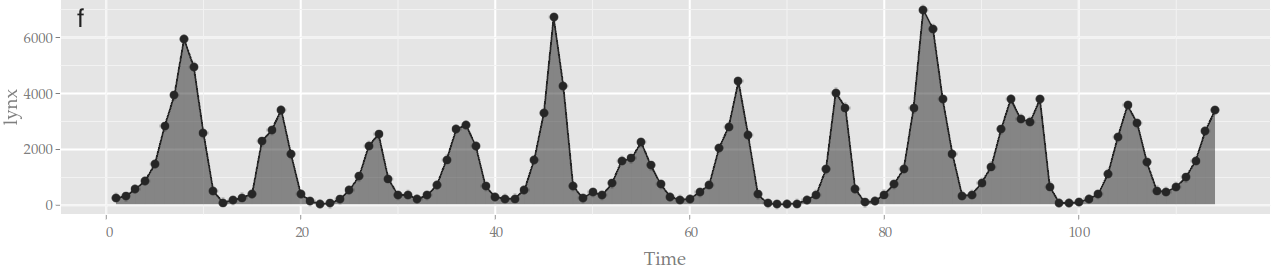
\includegraphics[width=0.8\textwidth]{graph/pipeline-18-original}} \\
%\multicolumn{2}{c}{\small{(g)}} \\
\multicolumn{2}{c}{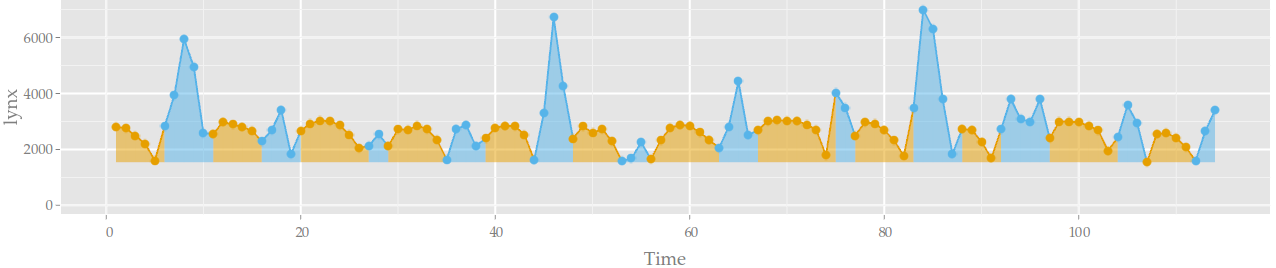
\includegraphics[width=0.8\textwidth]{graph/pipeline-18-mirrored}} \\
\end{tabular}
\caption{\label{fig:x-wrapping}Lynx trappings for 1821\textendash{}1934:
(a) Time series, (b \textendash{} d) stages of $x$-wrapping, matching
peaks, (e) faceted on the wrapped series, (f) area plot, (g) mirrored
on the mean, blue indicating values above the mean, and yellow below
the mean.  (Video illustrating these interactions is available at
\url{https://vimeo.com/112431547} and \url{https://vimeo.com/112432400}.)}
\end{center}
\end{figure}


\begin{center}
\begin{figure}[htp]
\begin{centering}
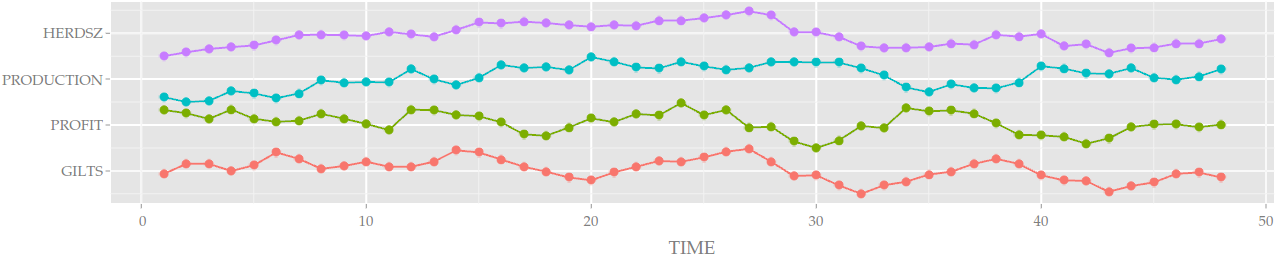
\includegraphics[width=0.98\textwidth]{graph/pipeline-17-original-wp-l}
\end{centering}

\begin{centering}
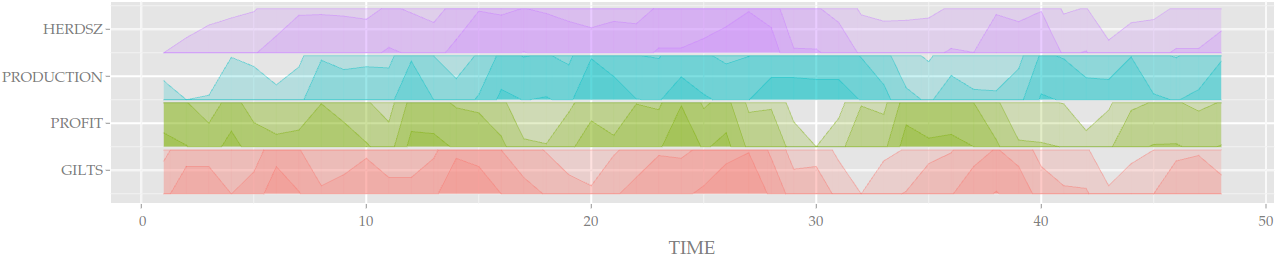
\includegraphics[width=0.98\textwidth]{graph/pipeline-17-ywrap-w}
\end{centering}

\caption{\label{fig:y-wrapping}Quarterly pig production for
1967-1978 in UK measured by five variables: (a) faceted, (b)
$y$-wrapped (see video at \url{https://vimeo.com/112435889}).
Profit and gilts seem slightly lag-related. Herdsz and
production may be related in a lag relationship also, but
neither is seasonal. In the $y$-wrapped version density indicates
the magnitude of values, and long periods of higher values,
like in herdsize are more visible. }
%Top: the original data faceted on variable. HERDSZ and
%PRODUCTION goes up slowly then down after the midway, and
%grows a little at the end. PROFIT and GILTS seems to show
%the seasonality with increasing variation. Bottom: $y$-wrapping.
%We see the gradually change for the first two variables and
%seasonal change for the latter two variables, also a leading
%pattern between PROFIT and GILTS. The video at
%\url{https://vimeo.com/112435889} demonstrates this wrapping.}
\end{figure}

\end{center}

\begin{center}
\begin{figure}[htp]
\begin{centering}
\begin{tabular}{cc}
%\multicolumn{2}{c}{{\scriptsize{ (a) not faceting}}}\tabularnewline
\multicolumn{2}{c}{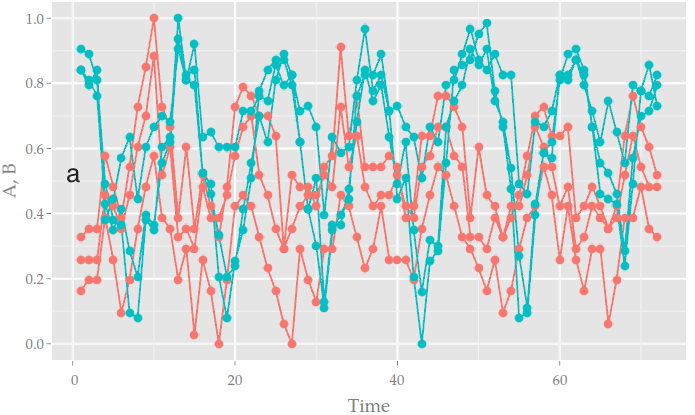
\includegraphics[width=0.48\textwidth]{graph/pipeline-14-1}}\tabularnewline
%{\scriptsize{ (b) faceting by variable}} & {\scriptsize{ (c) faceting by individual}}\tabularnewline
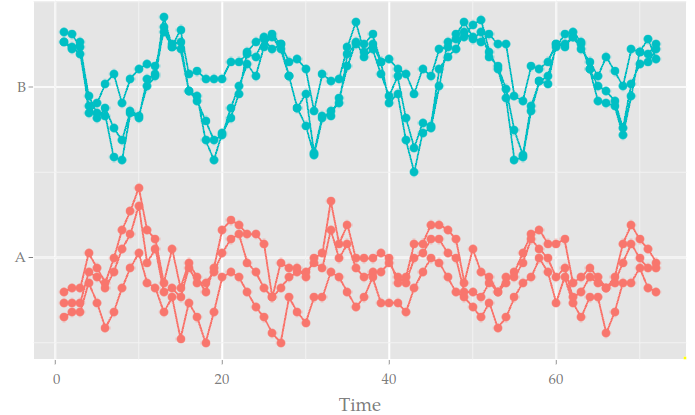
\includegraphics[width=0.48\textwidth]{graph/pipeline-14-2} & 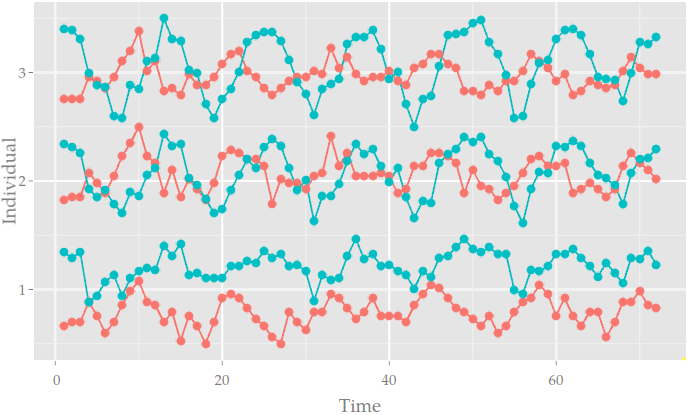
\includegraphics[width=0.48\textwidth]{graph/pipeline-14-3}\tabularnewline
%{\scriptsize{ (d) by variable then individual}} & {\scriptsize{ (e) by individual then variable}}\tabularnewline
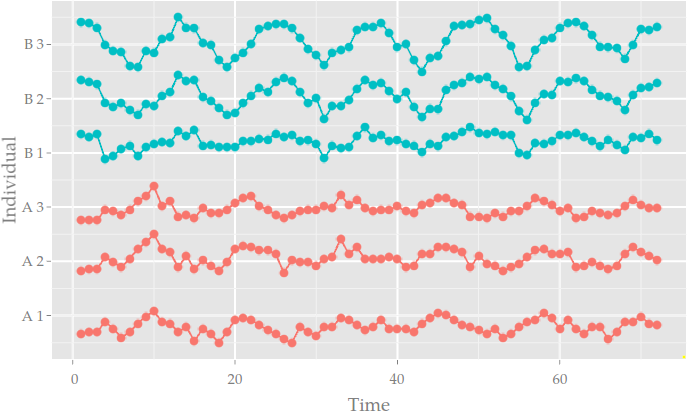
\includegraphics[width=0.48\textwidth]{graph/pipeline-14-4} & 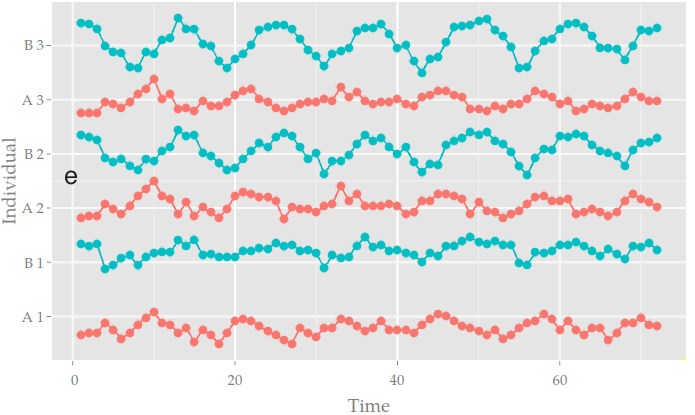
\includegraphics[width=0.48\textwidth]{graph/pipeline-14-5}\tabularnewline
\end{tabular}
\end{centering}

\caption{\label{fig:faceting-var-ind}Order of interaction matters when faceting with two variables and three individuals: (a) all series overlaid, color indicates variable, (b) facet first on variable (A, B),  (c) facet first by individual (1, 2, 3), (d) facets (b) by individual, and (e) facets (c) by variable. Both final configurations are useful: (d) supports the primary comparison of individuals, with variable comparisons secondary and (e) supports comparison of variables within individuals.  (Video footage illustration is available at \url{https://vimeo.com/112438919}.)}
\end{figure}

\end{center}


%\begin{figure}[htp]
%\begin{center}
%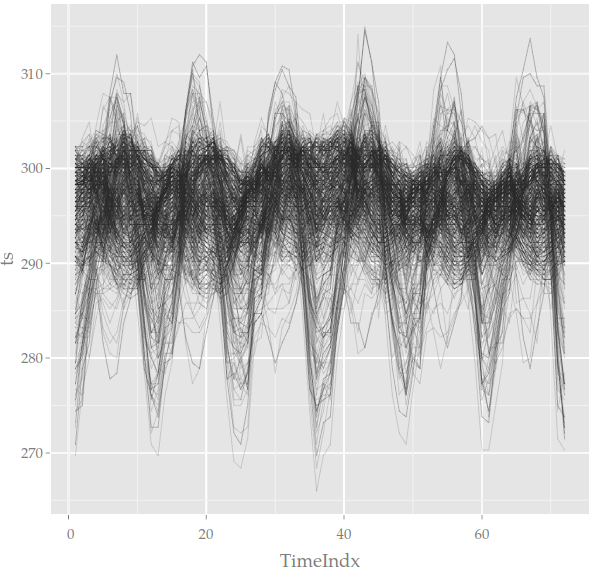
\includegraphics[width=0.38\textwidth]{graph/pipeline-24-1} 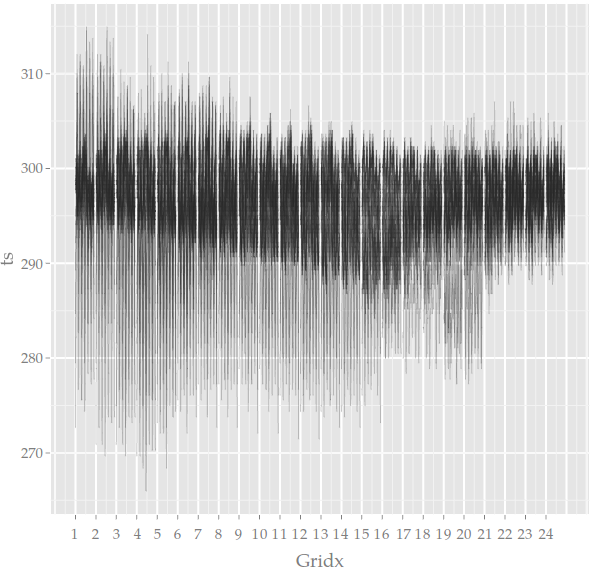
\includegraphics[width=0.38\textwidth]{graph/pipeline-24-3}
%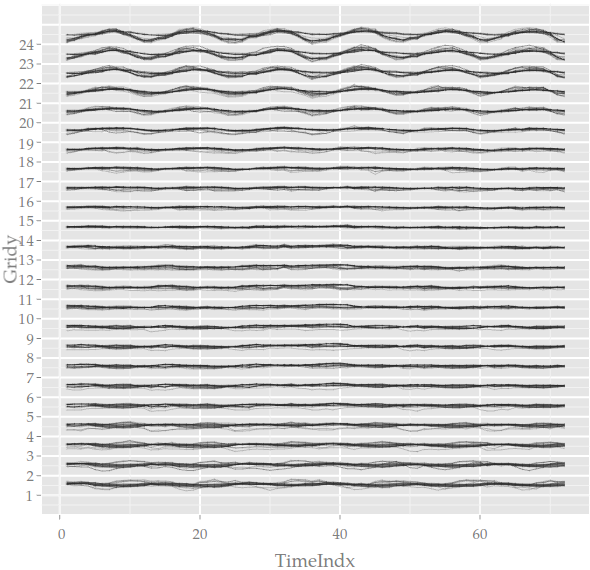
\includegraphics[width=0.38\textwidth]{graph/pipeline-24-2} 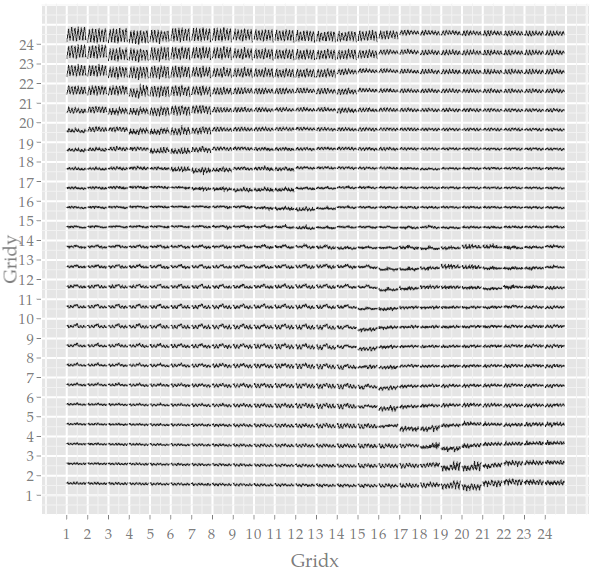
\includegraphics[width=0.38\textwidth]{graph/pipeline-24-4}
%\caption{\label{fig:faceting-2ind}Faceting on a tempo-spatial data set that have 72-month surface temperatures on a 24$\times$24 spatial grid
%\citep{murrell2010}.  (Top left) The mixed individuals.  (Top right) Faceting by longitudinal grid. There is more variation from the west areas than the east.  (Bottom left) Faceting by latitudinal grid.The north part is bumpier than the middle and south part.  (Bottom right) Faceting by longitude and latitude. An illustration of this facetting in both directions is shown in \url{https://vimeo.com/112503285}.}
%\end{center}
%\end{figure}


%\begin{center}
%\begin{figure}[htp]
%\begin{centering}
%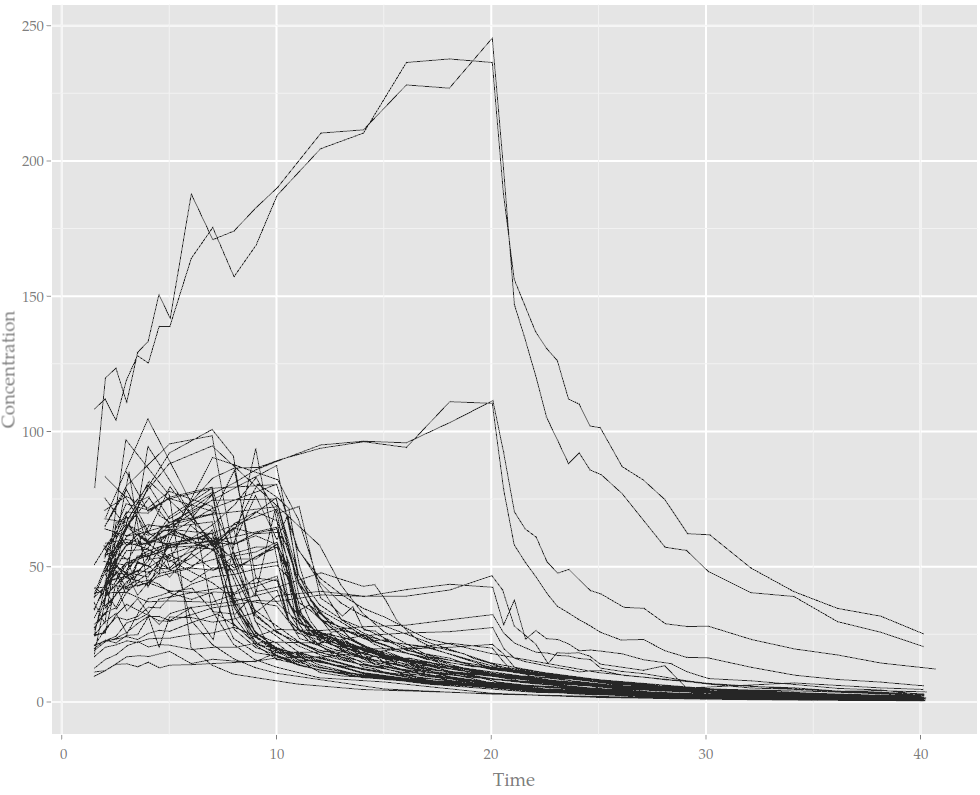
\includegraphics[width=0.4\textwidth]{graph/pipeline-25-1} 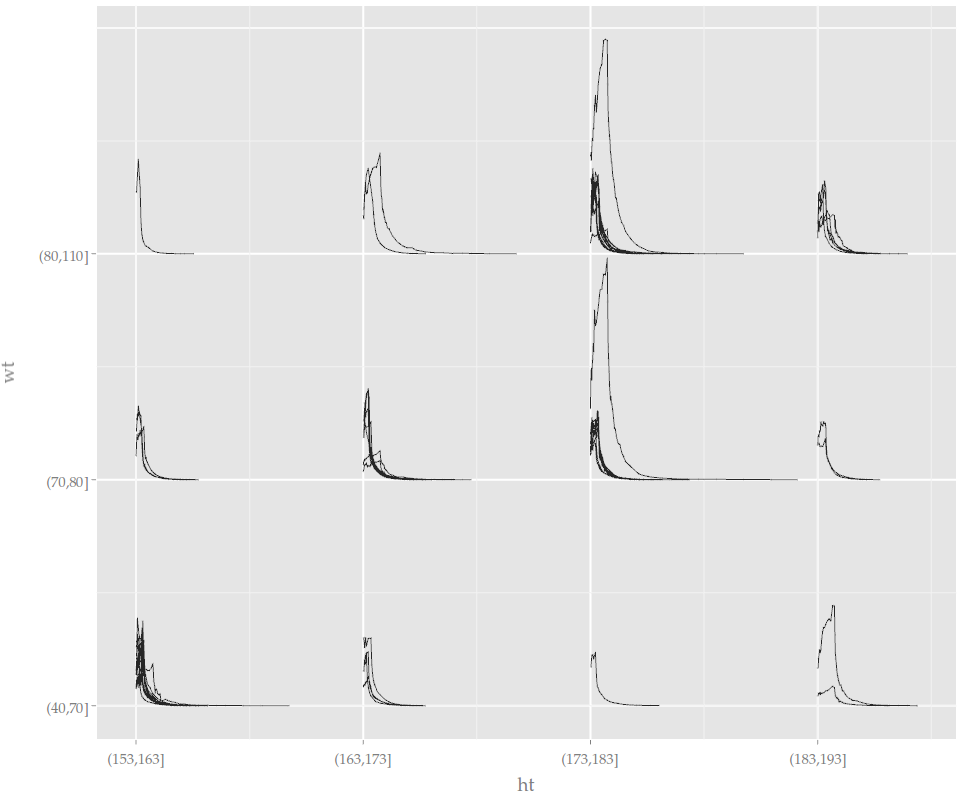
\includegraphics[width=0.4\textwidth]{graph/pipeline-25-3}
%\end{centering}
%\begin{centering}
%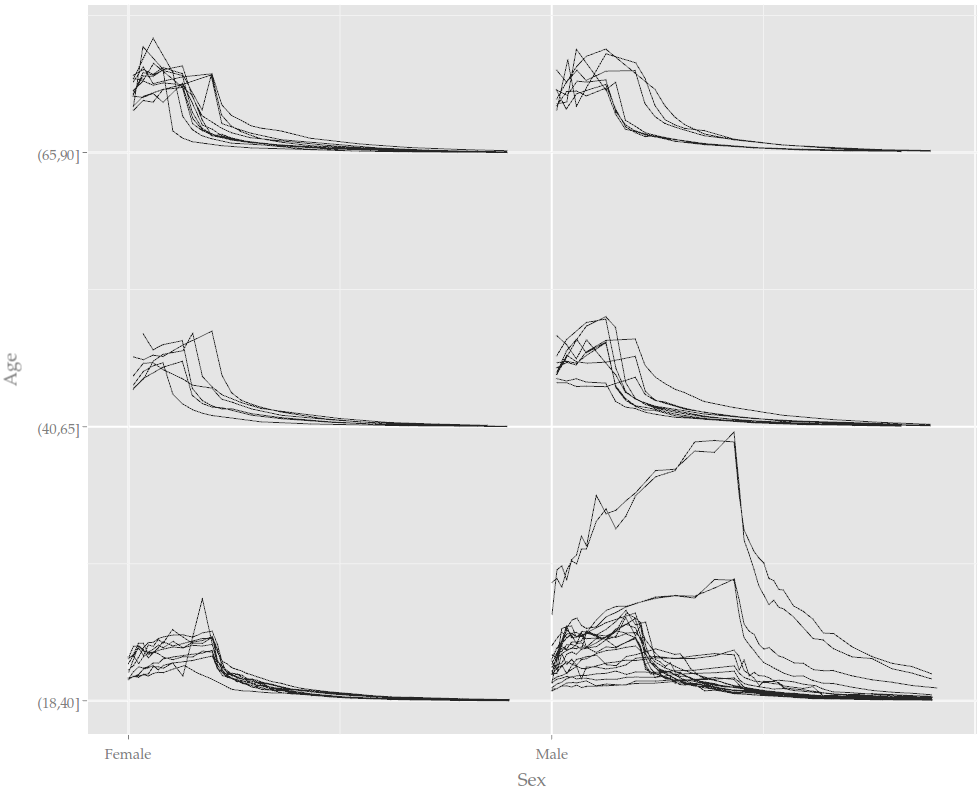
\includegraphics[width=0.4\textwidth]{graph/pipeline-25-2} 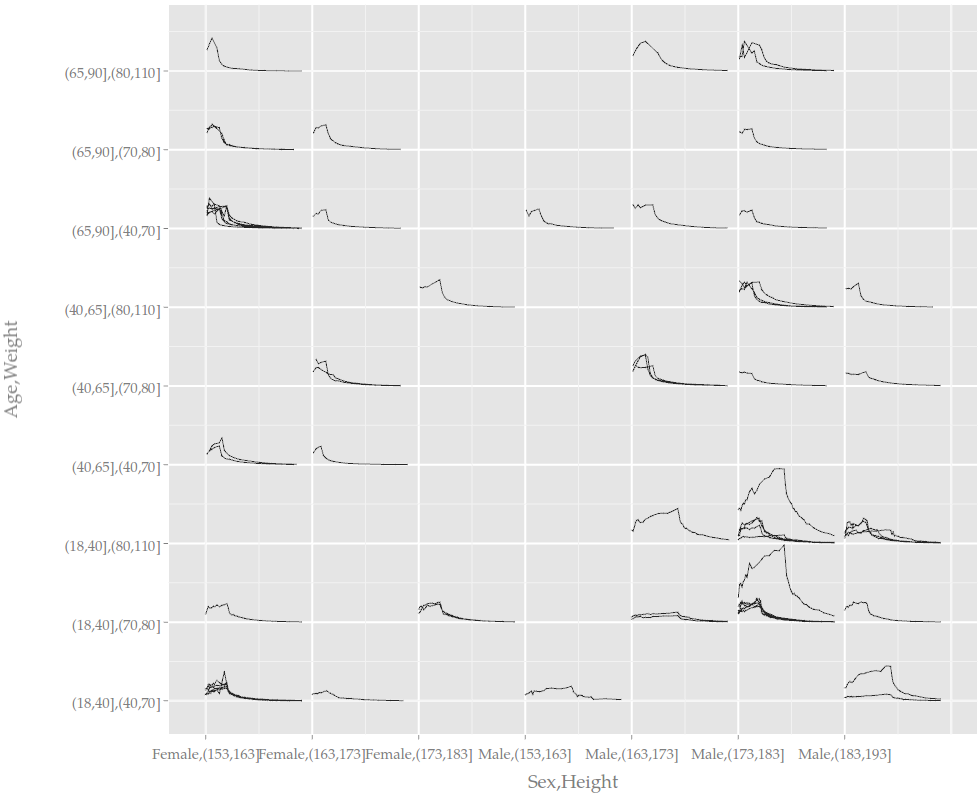
\includegraphics[width=0.4\textwidth]{graph/pipeline-25-4}
%\end{centering}
%\caption{\label{fig:faceting-4ind}Faceting on four categorical variables for a longitudinal data set  (pharmacokinetics of remifentanil, \citep{pinheiro2000mixed}). Sex and height are used in the horizontal direction, age and weight are used in the vertical direction.  (Top left) Original data without facetting.  (Top right) Faceted by height and weight.  (Bottom left) Faceted by sex and age.  (Bottom right) Faceted by sex and height horizontally, age and weight vertically. See the video at \url{https://vimeo.com/112509324} on how this works.}
%\end{figure}
%\end{center}


%\subsection{Considerations}
%An interactive system needs to include careful consideration of a number of aspects of the operations, which include accuracy after multiple actions, response time for the human user, and reverse actions. This section discusses ways to address these issues.


%\subsubsection{Additivity\label{sub:Additivity}}

% To make the interactions additive is not trivial when multiple
% types are allowed. It is important to know the current state,
% the initial state, and some intermediate states. When iteratively
% adding more of the same type of interaction, we can think of
% forward and backward movements. For these we need to know when
% to stop moving forwards, and knowing when the initial state is
% reached when backing up.  If a different interaction is started,
% keeping the state when this starts makes for a cleaner design.
% Figure \ref{fig:additive-interactions} explains why both the
% current and initial status are required by a faceting example.
% This will be re-visited Section \ref{sub:Two-procedures} after
% the formulas for different interactions are described.

% \begin{center}
% \begin{figure}[htp]
% \begin{centering}
% %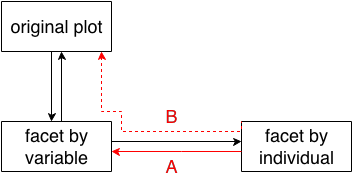
\includegraphics[width=0.5\textwidth]{graph/pipeline-20-additive-interactions}
% 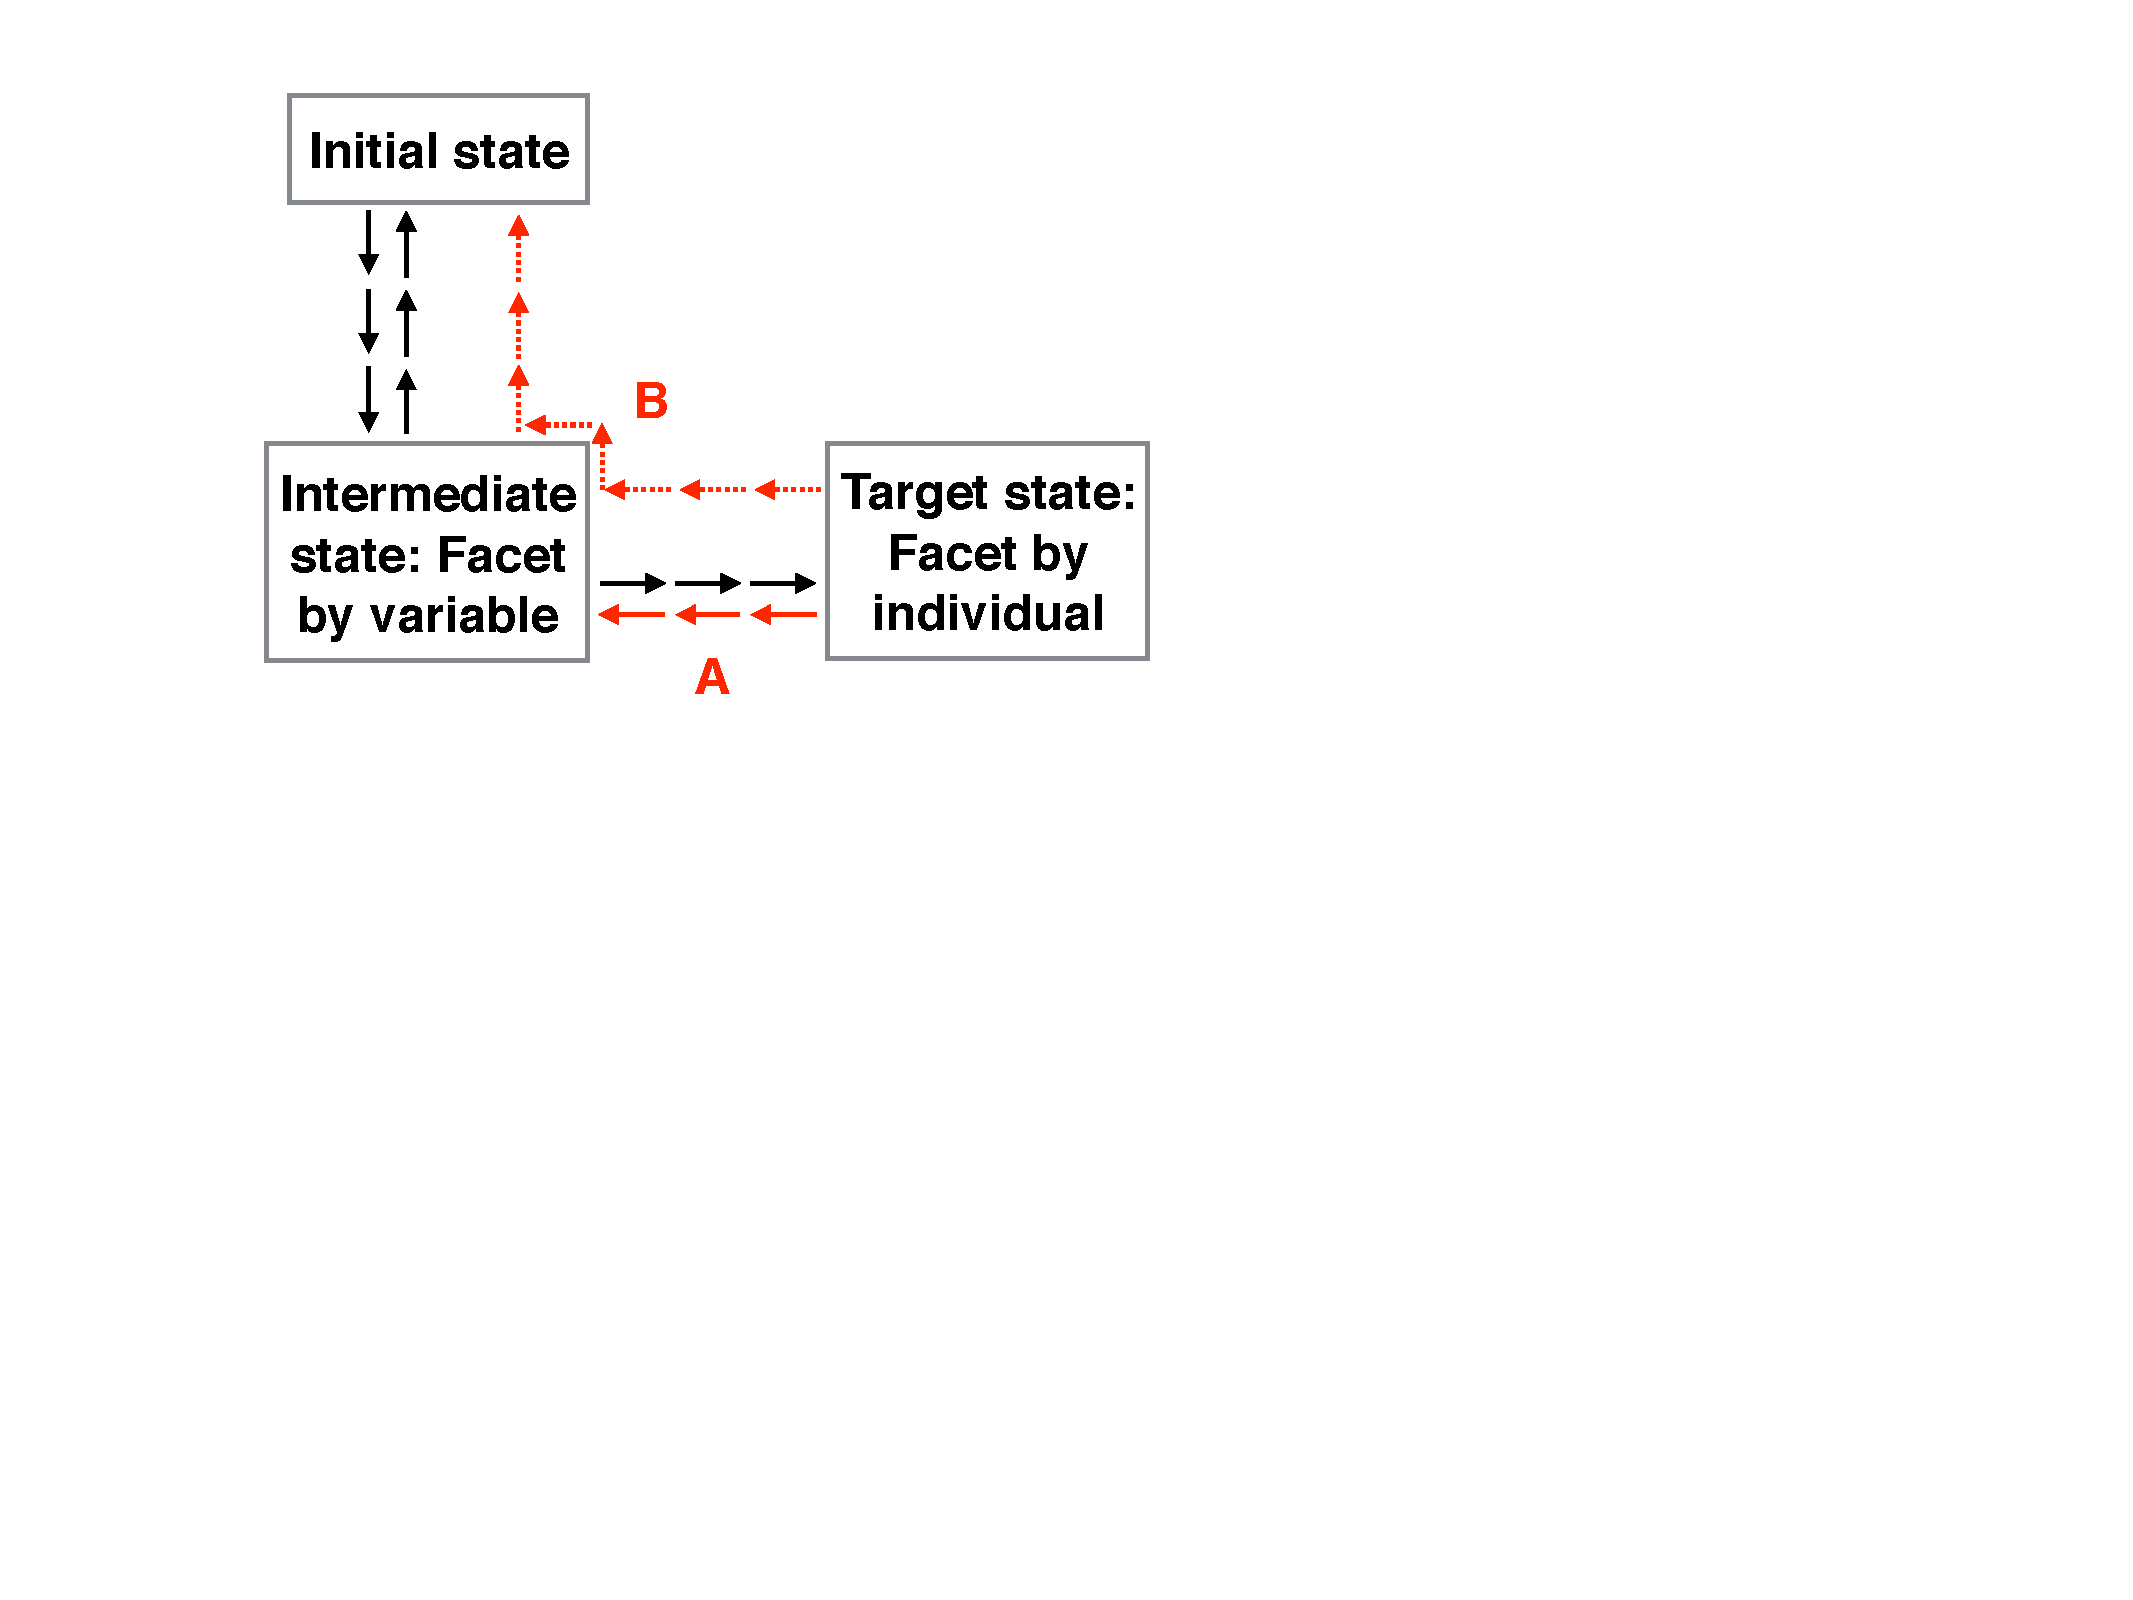
\includegraphics[width=0.5\textwidth]{graph/additivity.pdf}
% \par\end{centering}
% \caption{\label{fig:additive-interactions}
% Complications arise from multiple types of additive interactions, with transitional movement. to get from the initial state to the intermediate state and back is simple forward and backward actions. But when a further interaction is added, to get the final state, there are two ways to revert to the initial state, A and B. A is the cleanest approach, but requires saving the intermediate state. B can be completed because the forward states were achieved by adding increments to the point positions of the initial state, but might mean not seeing the intermediate state in the backwards transitions.}
% \end{figure}
% \par\end{center}

%\subsubsection{Transitional speed}

% Because the interactions happen in a transitional manner, from
% the initial state, through one or more intermediate states, to
% a target state  (e.g. Figure \ref{fig:smoothness}) there is a
% potential for a speed parameter. This parameter would control
% how quickly the plot changes to get to the target. There is
% some benefit for slow, smooth transitions, because small
% inconsistencies are revealed as series slide slowly past
% each other. There is also benefit to moving fast, to quickly
% get to a target state. It is also possible that there is no
% known, or fixed target state, in which case using the fast
% transitions could get to the neighborhood of the target state
% quickly, and using the slow transitions is easier to find the
% optimum when the state is close.

%For the interactions that modify the data coordinates, there will be a starting position, several  (or none) intermediate positions and a target position  (Figure \ref{fig:smoothness}). The starting position is the point coordinates before the interaction. The target position is the coordinates that maximize the effect of the interaction. The target position could either be known or unknown by the user. When it is known, any intermediate positions are not urgently needed, the interaction could be just a command to make the points jump from the starting position to the target. For example, with a known period, the user can wrap the series on the period directly. However, under many situations the target position is not known, and human intelligence are involved to seek the target. Then the intermediate positions are very important, and the step length between intermediate positions is crucial. The small steps make the interaction look smooth and not likely to miss the interesting phenomena, but are slow to reach the optimum. The big steps get close to the target quickly, but may miss it. Hence a gear to adjust the step length will be handy to control.


% \subsubsection{Bi-directional interactions and looping}
%
% Some interactions do not have an obvious target, e.g. wrapping.
% Then two types of designs for the movement direction are useful
% (Figure \ref{fig:interaction-direction}). A bi-directional design
% is smoother, because users can ease forward and backup on demand,
% to tune the state. However, it can be annoying, because it
% requires possibly too many commands and additional keyboard
% manipulation to return to the inital state. The bi-directional
% design works better for the interactions that change the
% coordinates or parameters further by repeating the command,
% e.g., horizontal or vertical wrapping. The other design, looping,
% is better for the interactions that jump to a parallel
% position. For example, in Figure \ref{fig:faceting-4ind} and
% its video, a longitudinal dataset is faceted by four categorical
% variables. The order of the categories on $x$ and $y$ axes can
% be rotated by some keyboard manipulations. Different orders make
% different positions, but they are all parallel with no position
% prior to the other in terms of the computational complexity.
% However, both styles of movement will need a quick return to
% an initial state, for convenience.

%but there must exist two manipulating commands for the forward and backward interactions. This is annoying to the users when there are many interactions because it doubles the number of commands. The loop design only needs one command, but a sudden change will happen in the transition from the last position to the starting position. Also, backing to the previous position will be a little painful by this design.

% \begin{center}
% \begin{figure}[htp]
% \begin{centering}
% %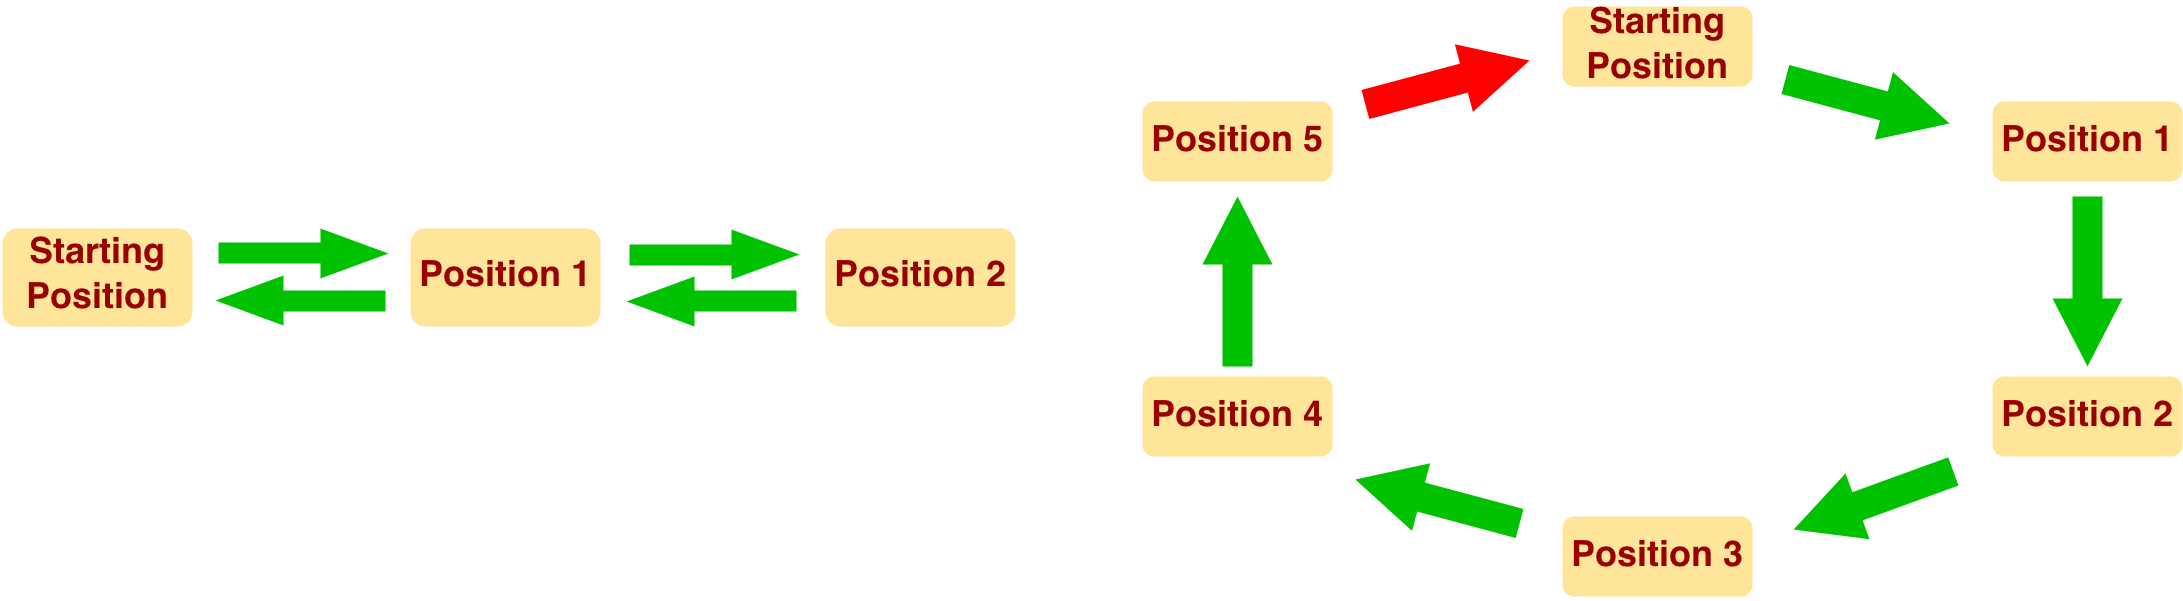
\includegraphics[width=0.98\textwidth]{graph/pipeline-21-directions}
% 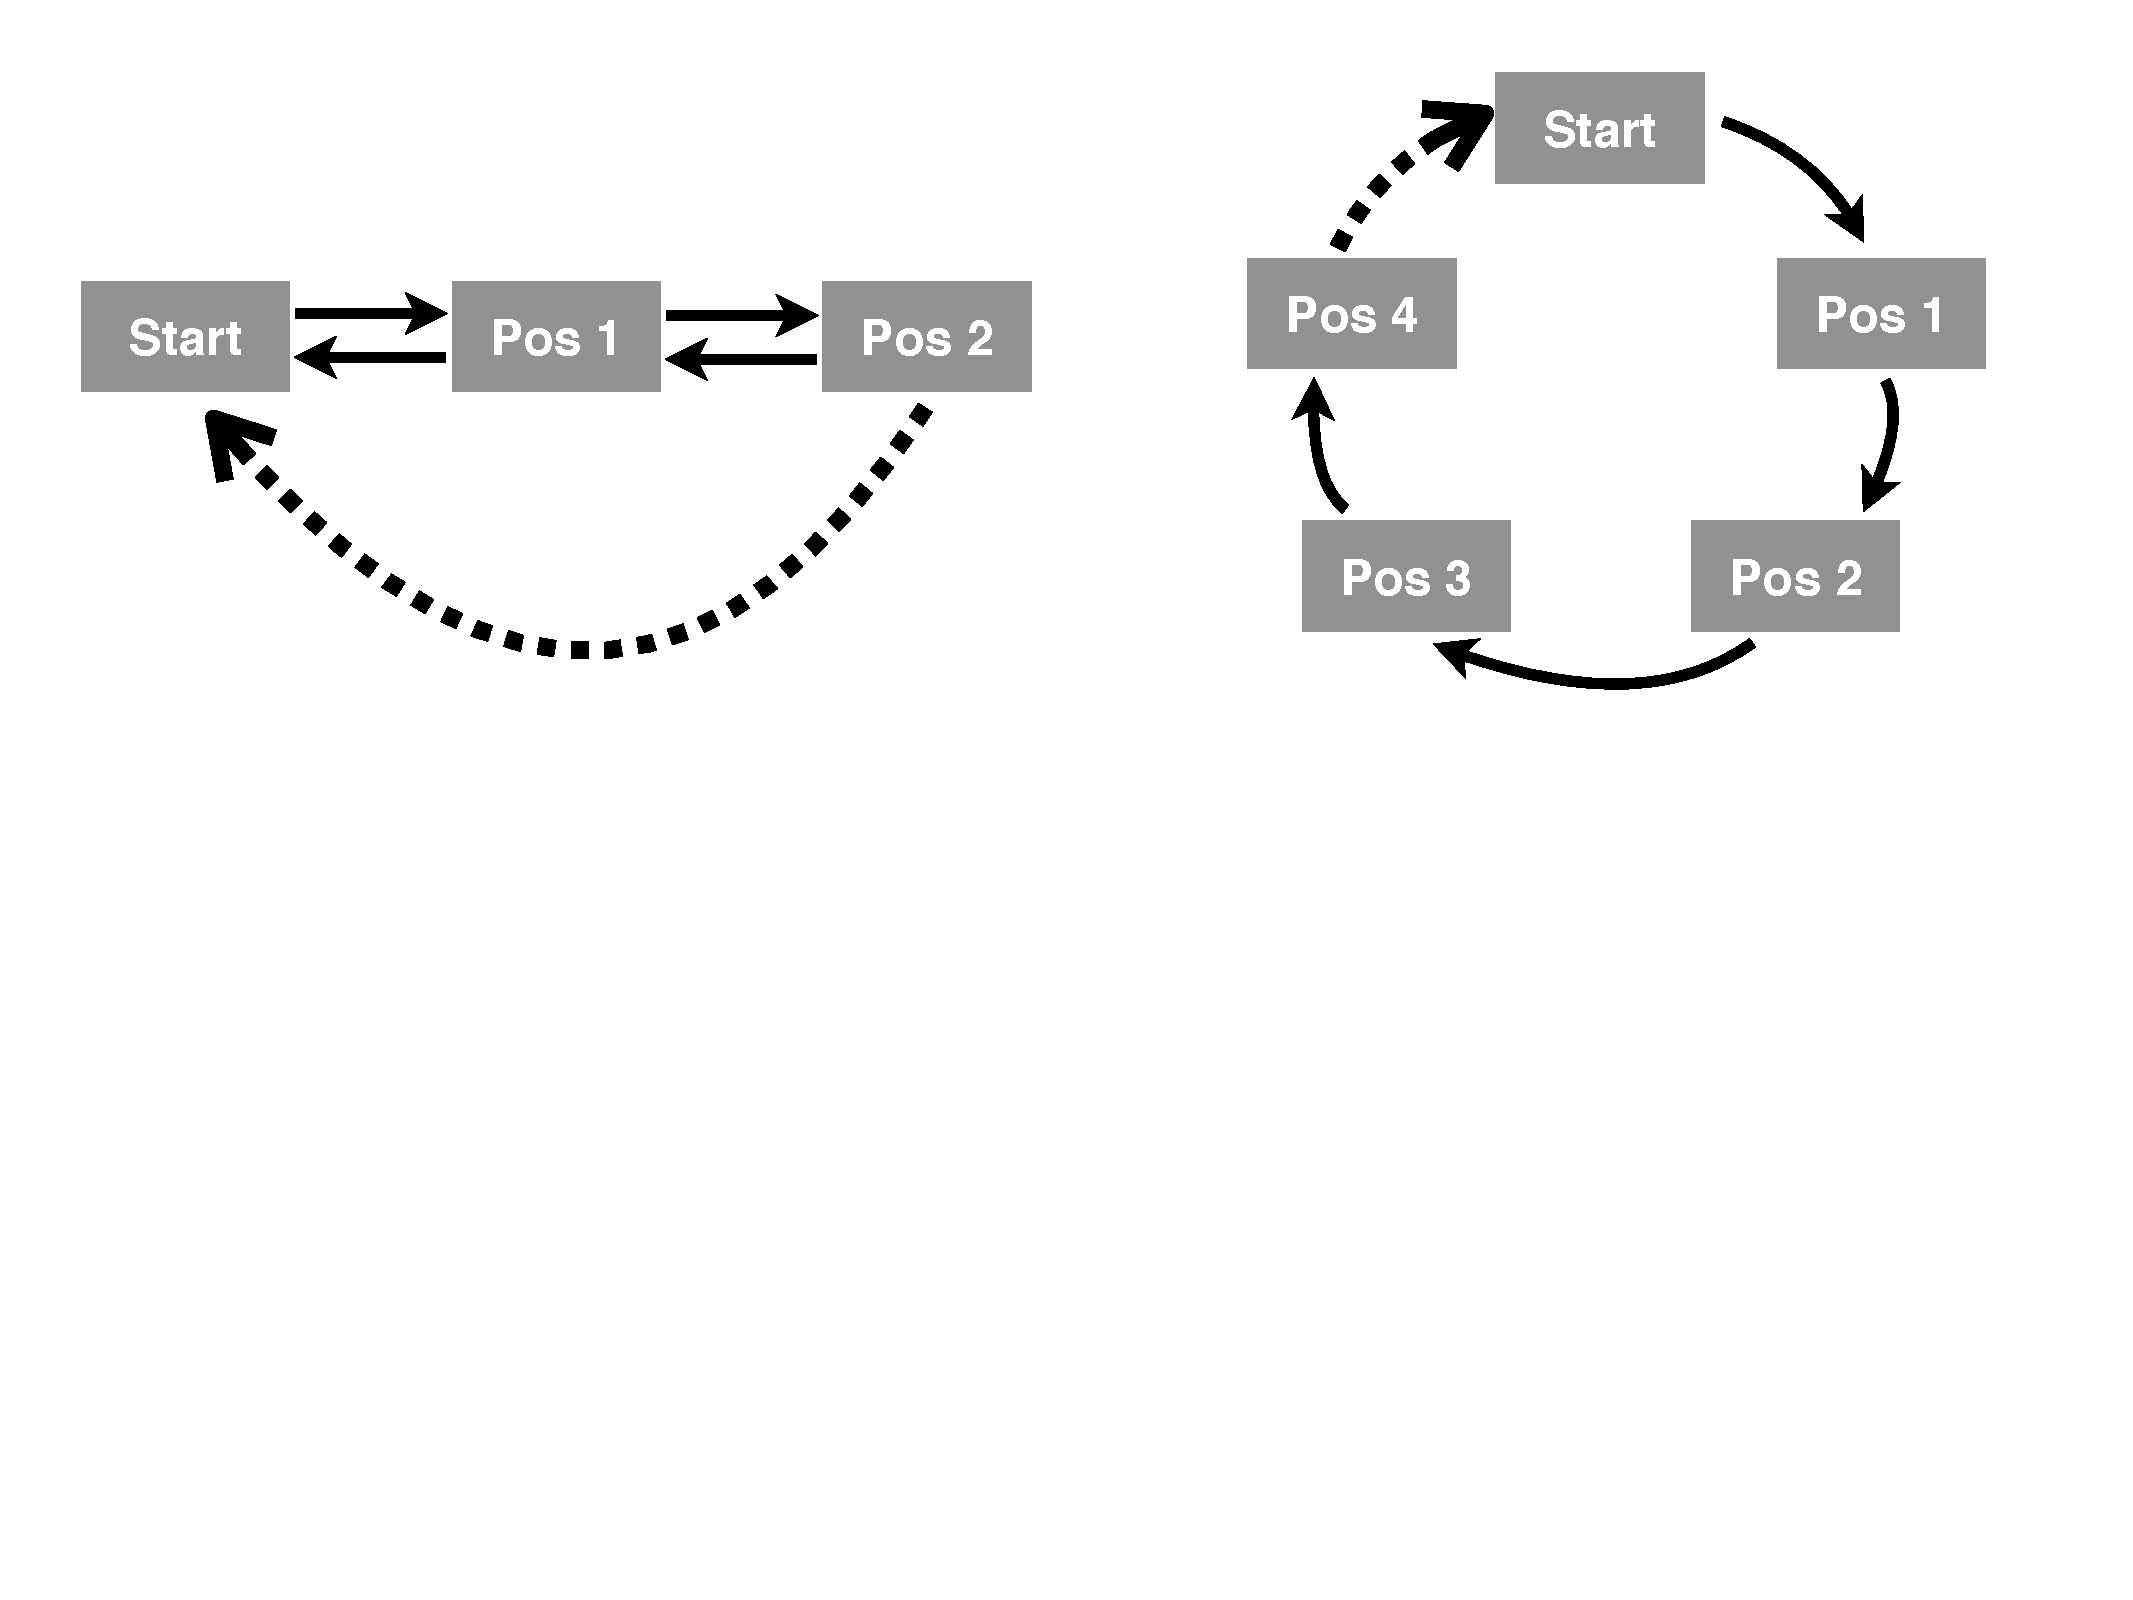
\includegraphics[width=0.70\textwidth]{graph/direction.pdf}
% \par\end{centering}
% \caption{\label{fig:interaction-direction}Two designs for the direction of
% interactions: (Left) bi-directional movement, and (right) loop.}
% \end{figure}
% \par\end{center}


\section{Display Pipeline\label{sec:Pipeline}}

\citet{wilkinson2000language, wilkinson2001nvizn, wilkinson2006grammar}
conceptualized and implemented a grammar of graphics that
carefully details a mapping of data to plots. It was extended
and implemented in \texttt{\textbf{ggplot2}} by \citet{ggplot2}. Data is
parametrized into elements, and assigned to graphical elements,
e.g. points, text, lines, polygons. \citet{wills2012visualizing}
made a simple extension for interactive graphics: \textit{``allow
the user to manipulate one of the two inputs, data or parameters,
and show the changes in the chart''}. Parameters, very generally,
describe a very broad class of characteristics, e.g. display
aesthetics like color or linetype, positional coordinates,
statistics such as bins, scales like limits or color ladders,
facets, and transformations. Much of what is needed to realize
the taxonomy of tasks for interacting with time series plots
can be considered to be data transformations. This section
describes the transformations required to perform shifting,
faceting, wrapping, and mirroring. Note that zooming is not
included because it does not change the relative distance between
the graphical elements. In \texttt{\textbf{cranvas}} zooming can
be manipulated simply by updating limits of the graphical device.

%Moreover, most of the parameters that Will mentioned are the graphical elements, like which elements to display, what color scheme to use, etc. In a more specific interactive graphics design, like the time series problem, the transform parameters need more attention.  Will did not give fully discussion for the last parameter type in his book, but he pointed out that ``\textit{the transforms are strongly data dependent}.'' In fact, the transformed data in the final display also strongly depend on the transform parameters, when there exist more than one type of transform. We will discuss how the interactions change both the transform parameters and data as follows. Note that the term $parameter$ will refer to the transform parameter, which could change the coordinates of the data.

\begin{figure}[htp]
\begin{center}
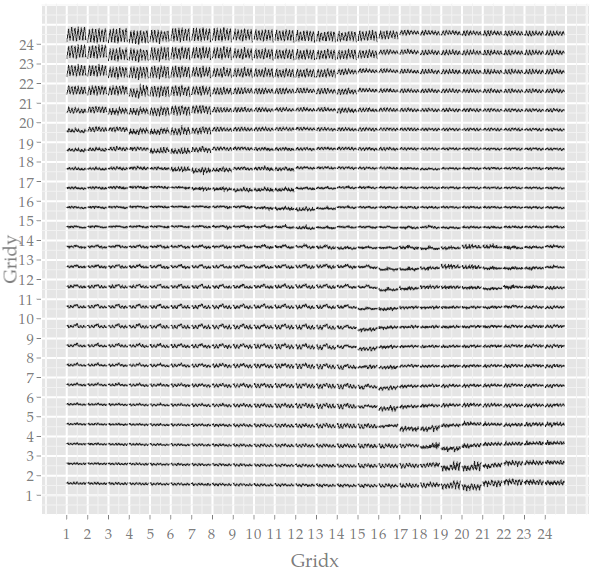
\includegraphics[width=0.45\textwidth]{graph/pipeline-24-4}\includegraphics[width=0.54\textwidth]{graph/pipeline-25-2}

\caption{\label{fig:faceting-examples}Faceting can be conducted bi-directionally: (left) by spatial grid for spatiotemporal data (\url{https://vimeo.com/112503285}), (right) by two covariates, sex and age, in longitudinal data (\url{https://vimeo.com/112509324}).}
\end{center}
\end{figure}

\begin{center}
\begin{figure}[htp]
\begin{centering}
\includegraphics[width=0.48\textwidth]{graph/pipeline-19-original}
\includegraphics[width=0.48\textwidth]{graph/pipeline-19-shifting}
\end{centering}
\caption{\label{fig:x-shifting}Illustration of shifting: three bottom series (variable A) are shifted horizontally to the right, to match the peak time with the top three series (variable B). (See also the video at \url{https://vimeo.com/112439923}.)}
\end{figure}
\end{center}

%\subsection{Generating interactions\label{interaction-formulas}}

Let $(\mathbf{x},\mathbf{y})$ denote the positional coordinates
for a temporal data set, where both are $n$-dimensional vectors
This notation is unconventional for time series, which typically
uses $x_t$ to represent the value records at time $t$, but it is
necessary for the graphical display because it allows us to think
about horizontal and vertical positions and adjustments to these
position. Because, many sequential interactions can be made, and
different types of interactions applied after each other, it is
useful to incorporate notation specifying these into the equations.
Let $\mathcal{I}$ be the temporal sequence of interactions,
e.g. $\{\textrm{facet},\textrm{wrap},\textrm{facet},
\textrm{zoom},\cdots\}$, and $j\in\mathcal{J}=\{1,2,\cdots,
J_{i}\}$ indicate the number of interactions made of type $i\in
\mathcal{I}$. Let $\mathbf{u}{}_{ij}=(u_{ij1},\, u_{ij2},\cdots)$
denote the user's input, e.g. key strokes,
$\mathbf{l}{}_{ij}=(l_{ij1},\, l_{ij2},\cdots, l_{ijn})$
be a line group indicator for each point, since some interactions might force new sets of lines,
$\mathbf{p}{}_{i}=(p_{i1},\, p_{i2},\, p_{i3},\cdots)$
be a parameter vector, e.g. a wrapping stop value of 3 points in series, and
$\mathbf{m}{}_{ij}=(\Delta\mathbf{x}{}_{ij},\,\Delta\mathbf{y}_{ij})$
denote the movements in $x$- and $y$- directions, where $i\in\mathcal{I}$
is an interaction type, and $j$ is the number conducted.
The new data coordinates are given by
\[
(\mathbf{x},\mathbf{y})_{s+\mathcal{I}_{ij}}=(\mathbf{x},\mathbf{y})_{s}+\mathbf{m}{}_{ij},
\]
where $s$ indicates the state before interaction.
The movement $\mathbf{m}{}_{ij}$ can be written as a function on $\mathbf{p}{}_{i}$,
$\mathbf{u}{}_{ij}$, $\mathbf{l}_{ij}$, $j$, and the inital
coordinates $(\mathbf{x},\mathbf{y})_0$,

\[
\mathbf{m}{}_{ij}=f_{i}(\mathbf{p}{}_{i},\:\mathbf{u}{}_{ij},\;\mathbf{l}_{ij},\; j,\; (\mathbf{x},\mathbf{y})_{0} ).
\]

\noindent These are the specific functional definitions used to generate the movement for the interactions available in \texttt{\textbf{cranvas}}.

%\subsection{Wrapping}
\subsection{Formulating the movements}

\begin{itemize} \itemsep 0in

% Figure \ref{fig:x-wrapping} (except bottom right plot)
% illustrates the horizontal wrapping of the lynx trapping data.
% The default wrapping interaction, by clicking a keystroke,
% induces the point at the end of the series, to be
% cropped and moved to the very left side of the plot, at the
% same $x$-position as the first time point. With repeated keystrokes, the
% most recent elements of the series will be cropped and gradually
% wrapped onto the earliest elements. Only the $x$-coordinates
% are changed -- the $y$-coordinates remain unchanged.
\item Wrapping. The wrapping can be defined as an algorithm:

\begin{enumerate} \itemsep 0in
\item Shift the data values up, usually by 1
\item Check the new $x$-limits, if a point has value large than upper limit, crop it using modulus arithmetic
\item Points that are cropped, have their line group indicator incremented
\item Connect the points that have the same line group indicator, in time order.
\end{enumerate}

For simplicity, we assume that the difference between consecutive
time values is 1. Let $x_{(1)},\cdots,x_{(n)}$ be the sorted
$x$-coordinates of the $n$ points in the series, that is the
points in time order. The $x$-limits after $j$ keystrokes for
$x$-wrapping will be reset to $(x_{(1)}, x_{(n-j)})$, so the
plot is rescaled accordingly. Let $\Delta_{n-j}=x_{(n-j)}-x_{(1)}+1$,
%then the new $x$-coordinate, $x^*$ of $x$ is
then the movements for $i=$ wrap are

\begin{eqnarray*}
\mathbf{m}{}_{ij} & = & \begin{cases}
(-\left(\left\lceil \frac{\mathbf{x}-x_{(1)}+1}{\Delta_{n-j}}\right\rceil -1\right)\times\Delta_{n-j}, \; 0) & 1\leq j \leq n-3 \\
(-\left(\left\lceil \frac{\mathbf{x}-x_{(1)}+1}{\Delta_3}\right\rceil -1\right)\times\Delta_3, \; 0) & j\ge n-2
\end{cases} \\
\end{eqnarray*}

where $\left\lceil \frac{\mathbf{x}-x_{(1)}+1}{\Delta_{n-j}}\right\rceil$
is equivalent to the line group indicator $\mathbf{l}{}_{ij}$.
The derivation of the formula, generalized cases for a faster
wrap and irregular time series can be found in Appendix
\ref{sub:appendix-wrapping}.

Movements from the $y$-wrapping on the $y$-direction,
as shown in Figure \ref{fig:y-wrapping}, could be obtained
by similar formulas. It is messier to realize because the
$y$-values are typically not in a sequential order which
means that more structural components need to be added to
the data to actually draw the wrapped series. Some of the
issues are discussed later in this paper.


%\subsection{Faceting}

%\begin{center}
%\begin{figure}[htp]
%\begin{centering}
%\includegraphics[width=0.32\textwidth]{graph/pipeline-22-original}
%\includegraphics[width=0.32\textwidth]{graph/pipeline-22-smooth}
%\includegraphics[width=0.32\textwidth]{graph/pipeline-22-jump}
%\end{centering}
%\caption{\label{fig:smoothness}Three positions of the faceting. Left panel is the starting position, center is an intermediate position with area layer, and right is the target position. There is some benefit for slow, smooth transitions, because small inconsistencies are revealed as series slide slowly past each other. There is also benefit to moving fast, to quickly get to a target state. See the video at \url{https://vimeo.com/112528131} to see the smooth transitions.}
%\end{figure}
%\end{center}

%In Figure \ref{fig:smoothness}, the interaction type $i=$ facet by individual. The plot in the center panel is obtained from the plot in the left panel by three repeated user actions, $j=3$. The plot in the  right panel appears after 20 repeated user actions from the plot in the left panel, $j=20$. When $j>20$, the plot will remain the same, since the series are already fully split. The threshold 20 is got by the
\item Faceting. When $i=$ facet by individual, with an initial setting of the
parameter $p_{i1}\in (0,1)$, which means that every hit on the
key will lift the $l$th standardized line by $(l-1)\times p_{i1}$,
the movements are
% Hence for $j\in\mathcal{J}$,
% \begin{eqnarray*}
% \mathbf{m}{}_{ij} & = & \begin{cases}
%  (0,\;0.05\, (\mathbf{l}{}_i-1)\, j) & 1\leq j<20,\\
%  (0,\; \mathbf{l}{}_i-1) & j\ge20.
% \end{cases}
% \end{eqnarray*}
% We can also generalize the equation above by
\begin{eqnarray*}
\mathbf{m}{}_{ij} & = & \begin{cases}
 (0,\; p_{i1}\, (\mathbf{l}{}_i-1)\, j) & 1\leq j<\frac{1}{p_{i1}},\\
 (0,\; \mathbf{l}{}_i-1) & j\ge\frac{1}{p_{i1}}.
\end{cases}
\end{eqnarray*}
%where $p_{i1}\in (0,1)$.

The example shows that $\mathbf{m}{}_{ij}$ is a function of $\mathbf{p}{}_{i}$,
$j$, and $\mathbf{l}_{ij}$, where $\mathbf{l}_{ij}=\mathbf{l}{}_i$ in this example
means that the line indicator for faceting is free from $j$.
More details on faceting by variable and period can be
found in Appendix \ref{sub:appendix-faceting}.


%\subsection{Mirroring}

\item Mirroring. To realize the interaction shown in Figure \ref{fig:x-wrapping} (g),
firstly we need to point the divider -- mean in this example.
Hence for $i=$ mirroring, the divider parameter
$p = \frac{1}{n}\sum_{d=1}^{n}y_d$. Then by $j\in\mathcal{J}$
hits on some triggering key, the movements are
\begin{eqnarray*}
\mathbf{m}{}_{ij} & = & \begin{cases}
(0, \; p+\max(p-\mathbf{y},\,\mathbf{y}-p)-\mathbf{y}) & j=1,3,5,\cdots \\
(0,0) & j=2,4,6,\cdots
%\end{cases}\\ & = & \begin{cases}
%(0, \; \max(2p-2\mathbf{y},\,0)) & j=1,3,5,\cdots \\
%(0,0) & j=2,4,6,\cdots
\end{cases}
\end{eqnarray*}
Note that if the mirroring is revisited after some other interactions,
then the count of $j$ should not be reset.

%\subsection{Shifting}

\item Shifting. Figure \ref{fig:x-shifting} illustrates
shifting the series, which is used to compare one series
against another. The user input uses $\mathbf{u}{}_{ij}$,
since the user can drag the
series horizontally to any position. The starting point
$u_{ij1}$ and end point $u_{ij2}$ of dragging on the $x$-axis,
as well as the selected series $u_{ij3}$ are the input from the user.
The horizontally shifting will not change $y$-coordinates, so for
$i=$ $x$-shifting and $j\in\mathcal{J}$, we have
\begin{eqnarray*}
\mathbf{m}{}_{ij} & = &
((u_{ij2}-u_{ij1})\times I\left\{ \mathbf{l}{}_{ij}=u_{ij3}\right\}, \; 0),
\end{eqnarray*}
where $I$ is the indicator function.

\end{itemize}


\subsection{Additivity of interactions\label{interaction-addition}}

Most of the interactions could be considered to be additive.
%That means interaction A can start at any status of interaction B.
Figure \ref{fig:faceting-var-ind} shows an example, where two
different results are generated by different ordering of interactions.
Faceting on individual is done after faceting on variable, with the
process following panels (a) $\rightarrow$ (b) $\rightarrow$ (d).
Faceting on variable after individual, as in the process (a)
$\rightarrow$ (c) $\rightarrow$ (e), produces a different
configuration of the time series. The additive application of
interactions is not commutative. Both results are useful, because
each facilitates a different type of comparison of the series,
using proximity. Plot (d) enables the comparison of individuals,
within variables, while plot (e) enables the comparison of series
within individual. It is also interesting to
note that wrapping vertically after mirroring, will result in
a horizon graph, like Figure \ref{fig:horizontal-axis} (f).
%Figure \ref{fig:faceting-period} shows another example of
%additivity: from the left to right, horizontal wrapping is
%followed by faceting on period.
%Also, users should be able to select the points, query the information, and link to other graphs after any interaction.

The cumulative interactions could
entirely change both $x$ and $y$ coordinates of data.
For example, Figure \ref{fig:x-wrapping} firstly directs
75 steps of $x$-wrapping, and then a faceting by
period. That gives the eventual movement by
\begin{eqnarray*}
\mathbf{m} & = & (-\left(\left\lceil \frac{\mathbf{x}-x_{(1)}+1}{\Delta_{39}}\right\rceil -1\right)\times\Delta_{39}, \; \mathbf{l}{}_{facet}-1) \\
& = & (-(\mathbf{l}{}_{wrap,75} -1)\times\Delta_{39}, \; \mathbf{l}{}_{facet}-1) \\
& = & (-(\mathbf{l}{}_{wrap,75} -1)\times\Delta_{39}, \; \mathbf{l}{}_{wrap,75}-1).
\end{eqnarray*}

Note that $\mathbf{l}{}_{facet} = \mathbf{l}{}_{wrap,75}$
in this example, because the line group indicator for
faceting by period is given by the wrapping steps.

In some other cases, a combination of interactions may
only modify either $x$ or $y$ coordinates. Figure
\ref{fig:faceting-var-ind} (a $\rightarrow$ b $\rightarrow$ d)
shows a combination of faceting first by variable then
by individual. The final movement after the full split
of individuals would be
\[
\mathbf{m} = (0, \; (\mathbf{l}{}_{facet~by~variable}-1)\times \max(\mathbf{l}{}_{facet~by~individual})+(\mathbf{l}{}_{facet~by~individual}-1)).
\]
% Table \ref{tab:additive-faceting} takes the first point
% of each series as an example to show $y$ and the changes
% at the three stages.
%
% \begin{table}[h]
% \begin{center}
% \begin{tabular}{|c|c|cc|c||c||c|}
% \cline{1-2} \cline{5-7}
% $l_{variable}$ & $l_{individual}$ &  &  & $y$ at (a) & $y$ at (b) & $y$ at (d)\tabularnewline
% \cline{1-2} \cline{5-7}
% 1 & 1 &  &  & 0.16 & 0.16+(1-1)=0.16 & 0.16+(1-1)$\times$3+(1-1)=0.16\tabularnewline
% \cline{1-2} \cline{5-7}
% 1 & 2 &  &  & 0.33 & 0.33+(1-1)=0.33 & 0.33+(1-1)$\times$3+(2-1)=1.33\tabularnewline
% \cline{1-2} \cline{5-7}
% 1 & 3 &  &  & 0.26 & 0.26+(1-1)=0.26 & 0.26+(1-1)$\times$3+(3-1)=2.26\tabularnewline
% \cline{1-2} \cline{5-7}
% 2 & 1 &  &  & 0.84 & 0.84+(2-1)=1.84 & 0.84+(2-1)$\times$3+(1-1)=3.84\tabularnewline
% \cline{1-2} \cline{5-7}
% 2 & 2 &  &  & 0.84 & 0.84+(2-1)=1.84 & 0.84+(2-1)$\times$3+(2-1)=4.84\tabularnewline
% \cline{1-2} \cline{5-7}
% 2 & 3 &  &  & 0.90 & 0.90+(2-1)=1.90 & 0.90+(2-1)$\times$3+(3-1)=5.90\tabularnewline
% \cline{1-2} \cline{5-7}
% \end{tabular}
% \end{center}
% \caption{\label{tab:additive-faceting}$y$-coordinates of the
% first point on each line, at Figure \ref{fig:faceting-var-ind}
% (a) no faceting, (b) faceting by variable, (d) faceting by
% variable then individual.}
% \end{table}

\subsection{Incremental vs baseline operations\label{sub:Two-procedures}}

Calculations can be made incrementally or with respect to a stable state (baseline), which, respectively, stores multiple copies of data, or a single storage of the data with storage of movement.
\begin{enumerate} \itemsep 0in
\item Incremental: Let

\begin{eqnarray*}
s_{0} & = & \textrm{initial status},\\
s_{t+1} & = & s_{t}+u_{i1}.
\end{eqnarray*}
 Note that every new status is only one interaction after the previous
status. The coordinates are given by
\begin{eqnarray*}
 (\mathbf{x},\mathbf{y})_{s_{t+1}} & = &  (\mathbf{x},\mathbf{y})_{s_{t}}+\mathbf{m}{}_{i1}\\
\mathbf{m}{}_{i1} & = & f_{i} (\mathbf{p}{}_{i},\;\mathbf{u}{}_{i1},\;\mathbf{l}_{i1},(\mathbf{x},\mathbf{y})_{s_0})
\end{eqnarray*}

This procedure always computes the next position directly from the
current position. The change only depends on the corresponding interaction
parameters and the input. The current status is stored in the memory
and ready to use for the next step. This method is an intuitive
design for interactive graphs with few special
interaction types. For example, scatterplots in \texttt{\textbf{cranvas}}
can change the size and transparency of dots. The new size (or
transparency) is always calculated by the multiplication of the
current size (or transparency) and a constant. The constant is
greater than 1 if the aesthetic parameter is increasing, and
less than 1 if the parameter is decreasing. The exponential
growth of the parameter accelerates the change and reduces the
times of repeated interaction.

The advantage of this procedure includes the straightforward design,
the convenience of moving to the previous or next status, and the
efficiency of avoiding the recomputation. However,
when there are many special interactions that could transform the
data, we need to record both the initial and current data positions
of each interaction type in the stream $\mathcal{I}$, because
when moving backwards, we need to know when the initial state is
reached and then stop. Then for an interaction stream $\mathcal{I}$
of length $k$, at least $k+1$ phases $ ( (\mathbf{x},\mathbf{y})_{s_{0}}, (\mathbf{x},\mathbf{y})_{s_{t_{1}}}, (\mathbf{x},\mathbf{y})_{s_{t_{2}}}\cdots, (\mathbf{x},\mathbf{y})_{s_{t_{k}}})$
should be saved, where $t_{1},t_{2},\cdots,t_{k}$ are the time of
the end of interaction types $1,2,\cdots,k$. When the data set is
large, those copies will occupy too much memory. Also, the storage
and management of $\mathbf{u}{}_{i1}$'s and $\mathbf{l}_{i1}$'s
is messy. Another drawback is that numerical errors could be
introduced after the same number of forward and backward
interactions, due to the floating-point arithmetic calculation.

\item Baseline: To store the $k+1$ phases, we do not make $k+1$
copies of the data set, instead, the movement item is traceable. The
coordinates of any status can be computed by
\begin{eqnarray*}
 (\mathbf{x},\mathbf{y})_{s_{t}} & = &  (\mathbf{x},\mathbf{y})_{s_{0}}+\sum_{i,j}\mathbf{m}{}_{ij}\\
 & = &  (\mathbf{x},\mathbf{y})_{s_{0}}+\sum_{i,j}f_{i} (\mathbf{p}{}_{i},\;\mathbf{u}{}_{ij},\;\mathbf{l}_{ij},\; j,\; (\mathbf{x},\mathbf{y})_{s_0}).
\end{eqnarray*}
Note that when a new position is required, the calculation starts
from the initial position instead of the previous status. The movements
from the original to the current position are computed instantly.

The idea of baseline operation is not new. In the tour movement
of \texttt{\textbf{XGobi}} and \texttt{\textbf{GGobi}}, the target
position is calculated by the initial position and the projection
parameters that come from the auto-oriented settings or
user-oriented interactions \citep{cook1995grand, cook1997manual}.
However, the interactivities that we discussed in this paper is
more complex, because we need to consider the interaction stream
$\mathcal{I}$, but the tour movement does not need to.
When there is only one type of modification, the formulas in
Section \ref{sec:Pipeline}%interaction-formulas}
will provide the target position easily.
 But when different types of modifications
are mixed, the baseline method structures the computation well.

With this procedure we do not need to save the intermediate
positions of the data, but we have to save the inputs for movements.
Now the problem turns to: how to store the inputs including
$\mathbf{p}{}_{i}$, $\mathbf{u}{}_{ij}$, $\mathbf{l}_{ij}$, and $j$? The answer is,
to save $\mathbf{l}_{iJ_i}$ with the data, where $J_i$ is the largest
$j$ in each $i \in \mathcal{I}$. This is because $\mathbf{p}{}_{i}$
is fixed and $j$ is known, $\mathbf{u}{}_{ij}$ is usually a short array,
but $\mathbf{l}_{ij}$ is of the same length as the data, and depends
on other parameters like $\mathbf{u}{}_{ij}$. So the data frame that
we use to save the data includes not only the coordinates, point parameters
like size and color, but also the line group indicators $\mathbf{l}_{iJ_i}$.

The advantage of this procedure is apparent: we do not have
to save multiple copies of data, and it is a better way to manage
the data and parameters during the interactions. However, it is not a comprehensive solution. We assumed that the movements are additive, but this is not always desirable. When changes in type of interaction make calculations better performed on a mid-way state, then it is better to stop, use this state as the baseline and then continue adding movements to this state.


\end{enumerate}

\section{Linking\label{sec:Linking}}

Linking between plots is a critical component of using multiple linked
windows \citep{stuetzle1987plot} to explore data. \citet{xie2014reactive} describes
types of linking and how it is realized in \texttt{\textbf{cranvas}}.
It is possible to both self-link, which is important for temporal data,
and link on different data sources or aggregation levels, using
categorical variables. For the temporal and longitudinal data,
linking is complicated when there is the need for different forms of
the dataset or additional data. Two situations are discussed in
the following sections.

\subsection{Self-linking}

Self-linking is primarily used to highlight all of the points in a time series when any one is selected. It is the most common behavior that a user would use. When there are multiple time series, it may also be useful to link to all points representing values recorded at a particular time.

Data underlying multiple time series, as for most of the other
plots available in \texttt{\textbf{cranvas}}, are usually in
``wide data'' format (Table \ref{tab:wide-data}). One row contains
the values recorded for a particular time, and aesthetic
parameters are associated with each row. In this form if the
display shows the multiple series, then when a user selects
one point by brushing, all the points (values for V1, V2, V3)
for this time are highlighted. This form is not conducive to
selecting either a single point or an entire time series.

%The time series and longitudinal data are usually ``wide'', as for each time point, there are inputs from multiple variables. To explore the dependency of the variables regardless of the time, many graph types, like the scatterplot and parallel coordinates plot, can be applied. However, if we utilize the ``wide data'' directly to generate a mutaframe and plot the time series, then different variables must share the same point parameters as from the same observations, as explained in Table \ref{tab:wide-data}.

A more flexible format is provided by melting the data
into the ``long data'' format (Table \ref{tab:long-data}).
In this format it is easy to realize brushing and self-linking
in different ways: the user can select a single point, and
(1) only this point is highlighted, (2) all points for
that line (e.g. V1) are highlighted, or (3) all points
for that time are highlighted (Figure \ref{fig:self-linking}).
The latter two are achieved by treating the line group
indicator or ``Time'' as a categorical linking variable,
respectively. Brushing and self-linking also works for longitudinal data, because it is typically in long data format.


%It is not ideal to make all the dots upon the same time point look the same. To force them to be brushed or unbrushed simultaneously is even a worse design. Hence we need the ``long data'' to assign different properties to different points. Table \ref{tab:long-data} is the corresponding long data of Table \ref{tab:wide-data}.


\subsection{Linking between plots}

Linking between plots builds a reactive brushing chain that
when the data points on one plot are brushed, then they are
highlighted on all the plots. In the normal cases of
\texttt{\textbf{cranvas}}, data behind the plots is unique,
so the brush interaction will modify the parameter attached
to the data and trigger the listeners of plots to highlight
the corresponding part. However, linking between a time
series plot and other plots (Figure \ref{fig:linking-plots}) is different, because the
data to create the time plot is in the long data format,
while the data to create the other plots, like scatterplots
or histograms, are in the wide data format. Hence, a link
between the two data formats must be constructed.

\citet{xie2014reactive} delineated how to link two data
objects. First a linking variable must be pointed out, then two listeners
are attached on the two objects. If the \texttt{.brushed} parameter
switches in one dataset, then the listener is triggered. And if any
observations from the second dataset have the same value in the linking
variable as the first dataset, then the corresponding \texttt{.brushed}
parameter in the second dataset will be changed.

Note that the linking between wide data and long data is not a one-to-one
linking. ``Time'' is the linking variable between two formats.
In the direction from wide to long data, each entry in the
wide data can project to multiple entries in the long data. In the
opposite direction, an entry in the long data will map to one entry in
the wide data. The unbalanced linking could produce a problem (see 
Table \ref{tab:wide-long-linking} in the Appendix). This problem can be solved by cutting off the backward linking.

\begin{figure}[htp]
\begin{center}
\includegraphics[width=0.32\textwidth]{graph/pipeline-27-1}
\includegraphics[width=0.32\textwidth]{graph/pipeline-27-2}
\includegraphics[width=0.32\textwidth]{graph/pipeline-27-3}
\end{center}
\caption{\label{fig:self-linking}When a single point is brushed,
there could be three modes of highlighting: (left) only a single
point is highlighted; (center) all points for that series are
highlighted, by treating the line group indicators as the categorical
linking variables; (right) all points for that time are highlighted,
by using the time as a linking variable.}
\end{figure}

\begin{table}[h]
\small
\begin{center}
\begin{tabular}{ccc}
\begin{tabular}{|c|ccc|ll|}
\hline
\multicolumn{4}{|c|}{Variables} & \multicolumn{2}{c|}{Parameters}\tabularnewline
\hline
Time & V1 & V2 & V3 & \texttt{.brushed} & \texttt{.color} \tabularnewline
\hline
1 & 3.1 & 27 & 11.9 & FALSE & red \tabularnewline
2 & 3.4 & 23 & 12.5 & FALSE & blue \tabularnewline
$\vdots$ & $\vdots$ & $\vdots$ & $\vdots$ & $\vdots$ & $\vdots$ \tabularnewline
\hline
\end{tabular}
& &
\begin{tabular}{|c|ccc|ll|}
\hline
\multicolumn{4}{|c|}{Variables} & \multicolumn{2}{c|}{Parameters}\tabularnewline
\hline
Time & V1 & V2 & V3 & \texttt{.brushed} & \texttt{.color} \tabularnewline
\hline
1 & 3.1 & 27 & 11.9 & FALSE & red \tabularnewline
\red{2} & \red{3.4} & \red{23} & \red{12.5} & \red{TRUE} & \red{yellow} \tabularnewline
$\vdots$ & $\vdots$ & $\vdots$ & $\vdots$ & $\vdots$ & $\vdots$ \tabularnewline
\hline
\end{tabular}
\end{tabular}
\end{center}
\normalsize
\caption{\label{tab:wide-data}Basic tabular form of data underlying plot (left), think of this as the ``wide data'' format. Each row contains values recorded at one time point. The aesthetic parameters are associated with one time point. Brushing on this form will highlight the points for a particular time (right), three points if all three series are drawn. It is probably more desirable for the behavior to be different: that selecting a single point will highlight all the values for that series, or only a single point, which can be achieved by a data re-structuring.}
\end{table}

\begin{table}[H]%[htp]
\begin{center}
\begin{tabular}{|c|cc|ll||ll||ll|}
\hline
\multicolumn{1}{|c}{} & \multicolumn{2}{c|}{} & \multicolumn{2}{c||}{Single point}& \multicolumn{2}{c||}{All V1}& \multicolumn{2}{c|}{All Time$=2$}\tabularnewline
\hline
Time & Variable & Value & \texttt{.brushed} & \texttt{.color} & \texttt{.brushed} & \texttt{.color} & \texttt{.brushed} & \texttt{.color}\tabularnewline
\hline
1 & V1 & 3.1 & TRUE & red & \textcolor{red}{TRUE} & \textcolor{red}{yellow} & TRUE & red \tabularnewline
2 & V1 & 3.4 & \textcolor{red}{TRUE} & \textcolor{red}{yellow} & \textcolor{red}{TRUE} & \textcolor{red}{yellow} & \textcolor{red}{TRUE} & \textcolor{red}{yellow}\tabularnewline
1 & V2 & 27 & FALSE & red & FALSE & red & FALSE & red\tabularnewline
2 & V2 & 23 & FALSE & blue & FALSE & blue & \textcolor{red}{TRUE} & \textcolor{red}{yellow} \tabularnewline
1 & V3 & 11.9 & FALSE & red & FALSE & red & FALSE & red \tabularnewline
2 & V3 & 12.5 & FALSE & blue & FALSE & blue & \textcolor{red}{TRUE} & \textcolor{red}{yellow}\tabularnewline
$\vdots$ & $\vdots$ & $\vdots$ & $\vdots$ & $\vdots$ & $\vdots$ & $\vdots$ & $\vdots$ & $\vdots$ \tabularnewline
\hline
\end{tabular}
\end{center}
\caption{\label{tab:long-data}The ``long data'' format, which is called the melted form in \citet{reshape}. This format allows a lot of flexibility. The ``Variable'' column can be used as a categorical linking variable, so that all points corresponding to ``V1'' are highlighted, when any one is selected, or a single point can be highlighted in the simplest brushing style, by changing the parameters of just that row. It would also be possible to use this form to use ``Time'' as a categorical variable for linking, and highlight all values recorded at a particular time. }
\end{table}


\begin{center}
\begin{figure}[htp]
\begin{centering}
\begin{tabular}{cl}
\multirow{5}{*}[2.1in]{\includegraphics[width=0.45\textwidth]{graph/pipeline-28-1}}
& \includegraphics[width=0.48\textwidth]{graph/pipeline-28-2} \tabularnewline
& \tabularnewline
& \tabularnewline
& \includegraphics[width=0.4\textwidth]{graph/pipeline-28-3} \tabularnewline
& \tabularnewline
\end{tabular}
\end{centering}
\caption{\label{fig:linking-plots}Linking between different plots
for the Google Flu Trends data (\url{http://www.google.org/flutrends/}) from November 24, 2013 -- March 16, 2014.
(Left) Time series faceted by state (see \url{https://vimeo.com/112528131}
for the transition to the facets), (top right) choropleth map grey
scale indicating time of the peak in the series, light is earlier,
(bottom right) histogram of the number of searches. Two states in
the map are brushed, which highlights all flu searches from these
states in the time series and histogram.}
\end{figure}
\end{center}


\section{Querying}

In each of the examples, and plots shown the time axis is
simply drawn using consecutive integers. This is necessary
for convenience and generalizability. To know which actual
time value requires querying, by mousing over the display,
if labels have been set up in detail, the user can learn what
day, month, year or individual identifier is under the cursor.

\section{Conclusions and future work}

This paper describes how interactions can be added to temporal displays by using sequences of affine transformations. This approach proves a rich variety of ways to slice and dice temporal data to explore seasonality, dependence, trends, anomalies and individual differences. These interactive temporal displays can be embedded in a large interactive graphics software system, enabling linking between plots to explore more general data where temporal components are just one aspect of many. Not everything is solved in terms of additivity, speed and interaction direction, but most common actions are possible for reasonably sized data.

Optimal aspect ratio for temporal displays is an unsolved problem,
and is something that we have grappled with in the implementation.
According to \citep{cleveland1993} time series should be ``banked''
to 45$^o$, which means that on average the angle of the lines, in
comparison to the $x$- or $y$-axes is 45$^o$. This is computed and
used in the initial plots in \texttt{\textbf{cranvas}}, but as
wrapping and faceting are conducted it probably should be
re-calculated. Ideal integration of aspect ratio re-drawing with
plot interactions could be examined in new work.

%In this paper we reviewed the static and interactive graphics for the time series and longitudinal data and refined the framework of interactions. For the time dependent data, we elaborated the three-layer display and proposed five special interactions for data exploration and pattern examination. Facilitating these heavily data-transforming interactions requires a new conceptual framework, including the timely coordinates calculation procedure and the linking system that supports brushing under new coordinates. We introduced two procedures to transform data during the interactions, and the linking within and between plots, or between the original data and additional data. However, some issues are still open to further discussion, like the additivity, transfer speed, and the interaction direction.

Future work would extend the interactions to include transforming between euclidean and polar coordinates, and between time and frequency domains. Earlier work in Dataviewer \citep{BAHM88} allowed users to interactively lag time series to generate lag plots to explore auto-correlation. This could be reasonably be accomplished similarly to the interactions described here.

%In future, more special interactions would be needed for the time dependent data, for example, the transformation between euclidean and polar coordinates, and the transformation between time domain and frequency domain. Besides, some more interactive plots will be needed, for example, interactive lag plots to detect auto-dependence between the time series and their lagged versions.

Using data transformations to generate interactions is efficient but it assumes the components are ordinal. This is not necessarily true, for example, in the flu searches series (Figure \ref{fig:linking-plots}) were faceted on the categorical variable state. This requires that states are first recoded to numerical values. In R, this is implicitly alphabetical order. However, because the implementation is created in R, the factor levels can be re-ordered easily, enabling the recoding to numerical value to be quite fluid. In the flu searches example, the states were re-ordered by earliest peak of searches.

This paper focused on interactive graphics for multivariate time series and longitudinal data, but the ideas should extend some to other temporal-context data.

%Another issue that needs to be solved in future is the order of series after faceting. When faceting by variable or individual, an order is needed to sort the lines from top to bottom, from left to right. In the current work we use alphabetical order for sorting variables, and the default factor level order for sorting individuals. But the best order for visualization may be different. For example, in Figure \ref{fig:linking-plots}, sorting the states by the time of flu search peaks could better track the spatial trend of flu search, or flu eruption. In R language, users can manually change the factor levels for individuals before plotting, however, if they are not confident about the best order, there should be an interaction to switch between different orders.

%This paper aims at the time series and longitudinal data, but the ideas on how to assist data-transforming interactions can be applied to other interactive graphics too.

\section*{Acknowledgements}
This work was started with funding from Google Summer of Code,
then partially supported by an unrestricted fellowship from
Novartis, and by National Science Research grant DMS0706949.

\bibliographystyle{natbib}
\bibliography{cranvastime}

\newpage
\section*{Appendix}
\renewcommand{\thesubsection}{\Alph{subsection}}
\setcounter{table}{0}
\renewcommand{\thetable}{A\arabic{table}}
\setcounter{figure}{0}
\renewcommand{\thefigure}{A\arabic{figure}}

\subsection{Wrapping}\label{sub:appendix-wrapping}

Recall that $\Delta_{n-j}=x_{(n-j)}-x_{(1)}+1$,
then the new $x$-coordinate after $j$ keystrokes
for $x$-wrapping, $x^*$ of $x$ is
\begin{eqnarray*}
x^* & = & \begin{cases}
x_{(n-j)}  & \mbox{if~} x-x_{(1)}+1 \mbox{~mod}\Delta_{n-j} = 0\\
(x-x_{(1)}+1) \mbox{~mod}\Delta_{n-j} ~~+x_{(1)}-1 &  \mbox{o.w.}
\end{cases} \\
& = & \begin{cases}
x_{(n-j)}  & \mbox{if~} (x-x_{(1)}+1) \mbox{~mod}\Delta_{n-j} = 0\\
(x-x_{(1)}+1)-\left\lfloor\frac{x-x_{(1)}+1}{\Delta_{n-j}}\right\rfloor\times\Delta_{n-j}+x_{(1)}-1 &\mbox{o.w.}\\
\end{cases} \\
 & = &
(x-x_{(1)}+1)-\left(\left\lceil\frac{x-x_{(1)}+1}{\Delta_{n-j}}\right\rceil -1\right)\times \Delta_{n-j} +x_{(1)}-1 \\ & = &
x-\left(\left\lceil \frac{x-x_{(1)}+1}{\Delta_{n-j}}\right\rceil -1\right)\times\Delta_{n-j},
\end{eqnarray*}
enabling the movements for $i=$ wrap to be described as
\begin{eqnarray*}
\mathbf{m}{}_{ij} & = & \begin{cases}
(-\left(\left\lceil \frac{\mathbf{x}-x_{(1)}+1}{\Delta_{n-j}}\right\rceil -1\right)\times\Delta_{n-j}, \; 0) & 1\leq j \leq n-3 \\
(-\left(\left\lceil \frac{\mathbf{x}-x_{(1)}+1}{\Delta_3}\right\rceil -1\right)\times\Delta_3, \; 0) & j\ge n-2
\end{cases} \\
\end{eqnarray*}
or equivalently in terms of line group indicators as well as points as
\begin{eqnarray*}
\mathbf{m}{}_{ij} & = & \begin{cases}
(-(\mathbf{l}{}_{ij} -1)\times\Delta_{n-j}, \; 0) & 1\leq j \leq n-3 \\
(-(\mathbf{l}{}_{ij} -1)\times\Delta_3, \; 0) & j\ge n-2.
\end{cases}
\end{eqnarray*}
The line group indicator $\mathbf{l}{}_{ij}$ will depend on
the number of interactions $j$.

Sometimes it is useful to wrap the series faster. If you have
a long time series, it might be useful to make full year jumps.
This can be achieved with the above equations by setting the
sequence of $j$ to respect this period. In other instances it
may be useful to have a multiplicative wrapping so that it
looks like the series wraps faster and faster with each step.
That means every keystroke will send a different number of
points from the right to the left. The number of points
wrapped by the $j$th step, can be represented by the user
input parameter $u_{ij}$. Then the $x$-range after $j$ steps
is $(x_{(1)}, x_{(n-\sum_{a=1}^j u_{ia})})$, yielding
$\Delta_{n-\sum_{a=1}^j u_{ia}}=x_{(n-\sum_{a=1}^j u_{ia})}-x_{(1)}+1$, and
\begin{eqnarray*}
x^* & = & x-\left(\left\lceil \frac{x-x_{(1)}+1}{\Delta_{n-\sum_{a=1}^j u_{ia}}}\right\rceil -1\right)\times\Delta_{n-\sum_{a=1}^j u_{ia}}, \\
\mathbf{m}{}_{ij} & = & \begin{cases}
(-(\mathbf{l}{}_{ij} -1)\times\Delta_{n-\sum_{a=1}^j u_{ia}}, \; 0) & 1\leq \sum_{a=1}^j u_{ia} \leq n-3 \\
(-(\mathbf{l}{}_{ij} -1)\times\Delta_3, \; 0) & \sum_{a=1}^j u_{ia}\ge n-2.
\end{cases}
\end{eqnarray*}

If the user wants to skip all intermediate positions and use
only one jump to the fully wrapped position, %as shown in Figure
%\ref{fig:faceting-period} from the left to center panel,
then the new $x$-range will be $(x_{(1)}, x_{(p_{i2})})$, where
the parameter $p_{i2}$ is the length of period. Hence for $j\ge 1$,
\begin{eqnarray*}
x^* & = & x-\left(\left\lceil \frac{x-x_{(1)}+1}{\Delta_{p_{i2}}}\right\rceil -1\right)\times\Delta_{p_{i2}}, \\
\mathbf{m}{}_{ij} & = &
(-(\mathbf{l}{}_{ij} -1)\times\Delta_{p_{i2}}, \; 0).
\end{eqnarray*}

To generalize our case to the irregular time series, we
should specify a wrapping speed parameter $p_{i3}$, i.e.,
with every key stroke, the $x$-range is shortened by at
least $p_{i3}$. The wrapping speed parameter will determine
how many points are shifted every time, because if the
difference between largest two points is greater than
$p_{i3}$, then only one point is shifted; if the difference
is smaller than $p_{i3}$, then more than one points are
shifted. After $j$ steps, the total number of points
shifted is a function of $p_{i3}$ and $\mathbf{x}_0$.
Denote the function as $g_j$, so the new $x$-range is
$(x_{(1)},x_{(n-g_j(p_{i3},\mathbf{x}_0)})$, and the
movements can be calculated then.

% \begin{center}
% \begin{figure}[htp]
% \centerline{\includegraphics[width=0.9\textwidth]{graph/wrap-example.pdf}}
% \caption{\label{fig:x-wrapping-algorithm} Cartoon illustrating
% the $x$-wrapping. There are three consecutive wrapping
% steps. At step $j=1$ the $x$ value of the last point changes
% from 21 to 16, and the line group indicator increments to 2.
% At step $j=2$ the $x$ values of the last two points are changed,
% and both have line group indicators equal to 2.  The wrapping
% stop parameter was set to $p_{i1}=3$, which means that after
% one more step, $n-j=3$, the wrapping would stop because each
% series has only 3 points. In the actual implementation the
% scale of the horizontal axis is changed at each step so that
% the full plot width is used.}
% \end{figure}
% \end{center}

\subsection{Faceting}\label{sub:appendix-faceting}

For $i=$ facet by variable/period, one click will fully split
the variables, so $j$ does not matter. All lines should be
standardized between $[0,1]$ first, then the movement is given by
\[
\mathbf{m}{}_{ij} = (0,\; \mathbf{l}{}_i-1).
\]
Note that $\mathbf{l}{}_i$ in this case differs from
$\mathbf{l}{}_i$ in faceting by individual.

\subsection{Linking}

To cutoff the backward linking problem, generated by linking to different forms of the data, two signals are added respectively
in the listeners of the two data objects. When one listener
is triggered, the signal will be turned on until the listener
finishes its work. During this period, the other listener cannot work.
As in Table \ref{tab:wide-long-linking}, the arrow from  (b) to  (c)
will be cut off.


\begin{table}[htp]
\begin{center}
\begin{tabular}{c|cc|cc}
\multicolumn{5}{c}{(a) Long data format, used in time plots}\tabularnewline
\hline
Time & Variable & Value & \texttt{.brushed} & \texttt{.color} \tabularnewline
\hline
$\vdots$ & $\vdots$ & $\vdots$ & $\vdots$ & $\vdots$ \tabularnewline
\textcolor{red}{2} & \textcolor{red}{V1} & \textcolor{red}{3.4} & \textcolor{red}{TRUE} & \textcolor{red}{blue} \tabularnewline
2 & V2 & 23 & FALSE & blue \tabularnewline
2 & V3 & 12.5 & FALSE & blue \tabularnewline
$\vdots$ & $\vdots$ & $\vdots$ & $\vdots$ & $\vdots$ \tabularnewline
\hline
\end{tabular}
%\end{center}

%\begin{centering}
$\Downarrow$
%\end{centering}

%\begin{centering}
\begin{tabular}{c|ccc|cc}
\multicolumn{6}{c}{(b) Wide data format, used in other plots}\tabularnewline
\hline
Time & V1 & V2 & V3 & \texttt{.brushed} & \texttt{.color} \tabularnewline
\hline
$\vdots$ & $\vdots$ & $\vdots$ & $\vdots$ & $\vdots$ & $\vdots$ \tabularnewline
\textcolor{red}{2} & \textcolor{red}{3.4} & \textcolor{red}{23} & \textcolor{red}{12.5} & \textcolor{red}{TRUE} & \textcolor{red}{blue} \tabularnewline
$\vdots$ & $\vdots$ & $\vdots$ & $\vdots$ & $\vdots$ & $\vdots$ \tabularnewline
\hline
\end{tabular}
%\end{centering}

%\begin{centering}
$\Downarrow$
%\end{centering}

%\begin{centering}
\begin{tabular}{c|cc|cc}
\multicolumn{5}{c}{(c) Long data format, used in time plots}\tabularnewline
\hline
Time & Variable & Value & \texttt{.brushed} & \texttt{.color} \tabularnewline
\hline
$\vdots$ & $\vdots$ & $\vdots$ & $\vdots$ & $\vdots$ \tabularnewline
\textcolor{red}{2} & \textcolor{red}{V1} & \textcolor{red}{3.4} & \textcolor{red}{TRUE} & \textcolor{red}{blue} \tabularnewline
\textcolor{red}{2} & \textcolor{red}{V2} & \textcolor{red}{23} & \textcolor{red}{TRUE} & \textcolor{red}{blue} \tabularnewline
\textcolor{red}{2} & \textcolor{red}{V3} & \textcolor{red}{12.5} & \textcolor{red}{TRUE} & \textcolor{red}{blue} \tabularnewline
$\vdots$ & $\vdots$ & $\vdots$ & $\vdots$ & $\vdots$ \tabularnewline
\hline
\end{tabular}
\end{center}
\caption{\label{tab:wide-long-linking}Linking between the long and wide data
format may produce a problem. Suppose we start from brushing a point  (V1
at time 2) in the long data  (a). Then the listener of the long data
is triggered and changes the .brushed parameter for time 2 in the
wide data  (b). Then the listener of the wide data is triggered and
switches the .brushed parameter for all the observations at time 2
in the long data  (c), which will update (a) but make a conflict.}
\end{table}
%\end{center}

%\subsection{Additional linking issues\label{sub:Linking-of-the-addition}}

Besides the issue of wide data and long data, there are other datasets
created during the interactions that could produce some linking issues,
such as the follows.
\begin{itemize} \itemsep 0in
\item The polygon data from the area layer.
The area layer does not
only need the values in the time series, but also the baseline to
form many polygons. To draw the polygons, the data must be rearranged
in an order of polygon vertexes. Each polygon is made of four vertexes:
two from the time series and two from the baseline. Because the polygon
layer should listen to the point and line layers, the link between
the original data and the polygon data is one-way.

\item Copies of the dataset during the incremental operation.
When adopting the incremental procedure in Section
\ref{sub:Two-procedures}, the variations of original dataset will
be created with multiple stages of the interactions. However, these
additional datasets are not required to get linked, because we only
make the copies of the coordinates, not the properties. To use the
coordinates, we combine them with the properties in the last minute,
so there will not be any linking issues.

\item Additional areas from the vertical faceting.
The example of vertical faceting is shown in Figure \ref{fig:y-wrapping}
and Figure \ref{fig:Additional-data} explained how the interaction
creates the additional areas. In Figure \ref{fig:Additional-data},
the black dots are given by the time series, and the red dots are
created during the cropping step of faceting, by the choice of
cutting lines. The black and red dots are mixed in some order to
form the shaded polygons. Whenever a point is brushed, one, two,
or even more cropped polygons should be highlighted. Hence the
two-direction linking between the cropped polygons and points
should be constructed. Note that this is a one-to-$n$ mapping,
and the linking variable is the point ID, which should be assigned
to the polygons when the red dots are generated.

\begin{center}
\begin{figure}[htp]
\begin{centering}
\includegraphics[width=0.48\textwidth]{graph/pipeline-23-1}
\includegraphics[width=0.48\textwidth]{graph/pipeline-23-2}
\end{centering}
\caption{\label{fig:Additional-data}Additional data created from the vertical
faceting. The black dots are given by the time series, and the red
dots are created during the cropping step of faceting.}
\end{figure}
\end{center}

\end{itemize}

\end{document}
